%!TEX root = ../BoYu-Dissertation.tex
\graphicspath{{Figures/}}

\chapter{Case Study: Promoting Awareness in Emergency Response} % (fold)
\label{cha:case_studies}
This chapter demonstrates the utility of the event-driven awareness promotion approach through a case study in the context of the emergency response \footnote{Partially result of this case study has been reported in a recent paper in ISCRAM 2012 conference \cite{Yu2012}.}. This case study aims to demonstrate the value of the event-driven awareness promotion approach in facilitating the emergency response operations by improved team awareness. 

The analysis of the case study includes two evaluation methods that are commonly used in design-science research \cite{Hevner2004}:
\begin{enumerate}
	\item The \emph{scenario-based analysis} is used to understand different characteristics of the awareness phenomena, and then to demonstrate the strength of our awareness approach in detailed use cases (Section \ref{sec:promoting_awareness_in_the_scenario}). As argued in \cite{Hevner2004}, the scenario-based evaluation method is appropriate for innovative artifacts for which other forms of empirical evaluation may not be feasible. 
	\item The \emph{computational simulation} is conducted to simulate the knowledge updating processes in the scenario (Section \ref{sec:simulating_the_knowledge_updating}) by using the prototype system described in Chapter \ref{cha:system_implementation}. The results of the simulation validate the computational knowledge updating process, and show the expressiveness of the PlanGraph model in our approach to represent the three characteristics of awareness phenomena in our conceptual model.
\end{enumerate}

This chapter is structured as follow: we first present the current status of awareness support in emergency response operations, and then include the development of a concrete scenario that consists of four episodes to demonstrate the typical development trajectories that may happen in collaborative activities. This `problem scenario' \cite{rosson2001usability} describes the current practices in the emergency response operations and sets up the grounded unit of analysis for our computational approach. Next, we conduct a computational simulation of the four episodes in our prototype system, the EDAP platform. The analysis of the results shows the capability of using the PlanGraph model to understand the major characteristics of collaborative awareness as described in our conceptual model (Chapter \ref{cha:the_conceptual_framework}). Last, we demonstrate the key strengths of our approach to promoting the awareness processes in several concrete use cases, as it would be if EDAP platform was used to promote awareness in the scenario.

\section{Awareness support in emergency response} % (fold)
\label{sec:awareness_support_in_emergency_response}
Emergency is any natural or man-caused situation that results in or may result in substantial harm to the population or damage to property \cite{shen2004managing}. Emergency response is the collaborative activity of gathering resources and acting upon the problems immediately after an emergency happens. While the scope of emergencies can be very broad (e.g. biological, chemical, nuclear/radiological, incendiary, or terrorist), the emergency operations share some common characteristics that make them fit into the scope of collaborative activities discussed in this study:

\begin{enumerate}
	\item Emergency response is well recognized as a type of collaborative activities with a high level of complexity \cite{Turoff2004}. Emergency response usually involves multiple, distributed individuals and organizations to mitigate the impact of incidents that threaten public safety and the environment. During an emergency situation, workers rarely tackle tasks in an independent way. Instead, they find themselves working on a multitude of different activities, interleaving them in ways that seem best suited for getting their work accomplished given the practical pressures.
	\item Furthermore, exceptions to the planned responses are a common and critical factor in these activities. An unplanned-for contingency may have its genesis in numerous circumstances \cite{Mendonca2004}: an emergency situation may evolve, so that implemented plans are no longer applicable; it may be multi-faceted, requiring responding organizations to combine many plans in unexpected ways; and it may occur concurrently with other situations, thus creating resource shortages or outages.
\end{enumerate}

With the high level of complexity and contingency in emergency response operations, supporting awareness has been recognized as an important component of emergency response management (ERM) systems \cite{Turoff2004}. Situation awareness is a critical element of emergency decision making in a variety of operational contexts. Existing studies have shown that improved situation awareness can benefit operational effectiveness by facilitating the planning process \cite{Javed2011}, improving the quality and timeliness of decisions \cite{Blandford2004}, and offering better feedback on the appropriateness of actions arising from such decisions \cite{Chen2008}. With respect to supporting team-level awareness, research into and development of emergency response support has mainly focused on shared situation awareness \cite{Treurniet2012}, which has been considered as an essential prerequisite of an accurate collective picture of the emergency, and the basis of team decisions since they bring together and share individual perceptions, understandings, and predictions \cite{Javed2011}. However, the distributed nature of team-level awareness, i.e. the fact that awareness should be considered as a partly shared and a partly distributed understanding of a situation among team members, has not been well recognized and supported in existing emergency response management systems \cite{Treurniet2012}.

Current computational environments for awareness support in emergency response management favor the event-based awareness models for two reasons:

\begin{enumerate}
	\item The domain of emergency response has foundations in event driven task accomplishment \cite{Pottebaum2011}. Emergency response efforts are triggered by an incident, or a disaster, i.e. an ``event'' happening in the environment. To respond to the initial event, actors perform activities that add more events building up the situation. Decision makers have to react to these critical events for continuous response. Therefore the awareness they need is built up both from danger events as wells as emergency response events.
	\item Actors in the emergency response operations have to focus on information needed and the immediate situation factors that relate to the decisions and actions they are taking \cite{Turoff2004}. As a result, they have very limited attentional resources to actively monitor the environment and each other's work in order to pick up the awareness information peripherally. The event-based model has the advantage in pushing the information to the actors so that they do not need to switch their attentions to the periphery until the event are notified to them.
\end{enumerate}

Although much progress has been made to provide more effective event-based awareness support in emergency response operations with the integration of complex event-processing (CEP) engines (e.g. PRONTO \cite{Pottebaum2011} and PLAY projects \cite{Truptil2012}), the limitations of event-based models as we discussed in Section \ref{sec:the_state_of_art} also exist in the emergency response domain: 

\begin{enumerate}
	\item The effectiveness of event-based models largely depends on the quality of event subscriptions, which often requires considerable effort from the actors to explicitly manage. With the high level of complexity and contingency in emergency situations, existing event notification mechanisms either lead to too many irrelevant events notified to the actors, or the actors have to frequently modify subscriptions to adapt to their changing needs.
	\item The current event-based systems in the emergency response domain focus on the external events that are generated by physical sensors or complex events that are calculated by the rule-based event processing agent \cite{Pottebaum2011}, little support has been given to the social development of awareness, i.e. the internal events generated by the human actors during awareness transactions.
\end{enumerate}

In the following of this chapter, we describe a concrete emergency response scenario and then use it to argue how these limitations can be addressed in our event-driven awareness promotion approach.
% section awareness_support_in_emergency_response (end)

\section{An emergency response scenario} % (fold)
\label{sec:an_emergency_response_scenario}
For this case study, we consider a nuclear crisis scenario in which a large quantity of radioactive substance is accidentally released in the atmosphere, due to a critical accident in a nuclear plant. The multiplicity and diversity of actors involved, the volume and heterogeneity of information, the critical dependencies between actions as well as the dynamics of the environment make the situation more complex. 

This scenario is based on the document analysis from several government websites, including the National Response Framework \footnote{http://www.fema.gov/national-response-framework}, the Nuclear/Radiological Incident Annex to NRF \footnote{http://www.fema.gov/pdf/emergency/nrf/nrf\_nuclearradiologicalincidentannex.pdf}, NRC Incident Response Plan \footnote{http://www.nrc.gov/about-nrc/regulatory/incident-response.pdf}, as well as a collection of FEMA after action reports related to specific emergency exercise \footnote{http://www.nrc.gov/about-nrc/emerg-preparedness/related-information/fema-after-action-reports.html}. To simplify the analysis, however, we reduce the complexity of the emergency response operations significantly in this scenario, comparing with the real world situations as described in these documents.

In the following of this section, we first provide an overview of the scenario, with the major elements in the collaborative activity, i.e. the actors, resources, and actions, as well as the external events. Then we describe four concrete episodes in the scenario, reflecting the different developmental trajectories of the collaborative activity.

\subsection{Overview of the scenario} % (fold)
\label{sub:overview_of_the_scenario}

\paragraph*{Source of the incident} % (fold)
\label{par:source_of_the_incident}
The radiation leak in this scenario originates from the combination of two problems in a nuclear plan:
\begin{enumerate}
	\item Due to the wearing effect of time, a leak appeared in the steam generator. As a result, the water within the primary loop connecting the reactor and the steam generator, contaminated, spreads through the secondary loop.
	\item The throttle valve, a safety device of the secondary loop, opens due to the increased pressure inside the secondary loop. It does not respond to the manual bypass of the safety loop. As a result, the steam of the secondary loop, contaminated, escapes to the atmosphere.
\end{enumerate}
% paragraph source_of_the_incident (end)

\paragraph*{Actors} % (fold)
\label{par:actors}
To respond to the emergency caused by the radiation leak, many stakeholders are involved. The emergency operation center (EOC), in charge of operation, is formed with federal agencies, state and local public safety officials. Besides, firemen, policemen, and any other actors involved in the response process has one representative at the emergency operation center, to validate the feasibility of decisions, link with the field and ensure communication between actors. The EOC is distributed. Most of the decisions are made locally, where delegates are gathered, but decisions may also come from the national authority, state or local officials, or experts.

Besides the EOC, a large number of actors work in the filed to operate or support the nuclear crisis response. This includes (1) firemen to distribute iodine and search for victims in the impacted area, (2) decontamination and medical teams to assist victims, (3) transportation team to provide prompt delivery of personnel, equipment, and victims, (4) police to confine population and guide the evacuation, (5) and scientific team to survey radiation, provide meteorologic information, and assess the evolution of the situation.
% paragraph actors (end)

\paragraph*{Resources} % (fold)
\label{par:resources}
A variety of resources are used by the actors in the scenario to perform their tasks. Some of the resources are used to perform specific tasks, such as the measuring equipment used by the scientific team to survey radiation, and some are shared by multiple actions. For instance, the rescue vehicles can be used for transporting victims, and delivering actors or other resources. The resources can be `tools' such as the measuring equipment, and also be `objects', such as the victims that are manipulated by multiple actors in different tasks, such as decontamination, medical treatment, or transportation. 

Here we highlight several types of resources that are frequently in the four detailed episodes:

\begin{enumerate}
	\item The victims are the people in the impacted area that have be contaminated by the nuclear radiation and/or physically injured.
	\item In order to perform decontamination operations on the victims, several mobile decontamination stations have been set up, and are managed by a decontamination manager in the EOC. Each station includes several decontamination operators to monitor the resources (e.g. the rinse tanks) and perform the decontamination operations.
	\item Similarly, several mobile medical stations are also set up to perform medical treatment on the injured victims. The medical stations are managed by a medical manager in the EOC, and each of them includes several paramedics.
	\item Multiple rescue vehicles are available to provide prompt delivery of victims, equipment, and rescue personnel. Each vehicle is associated with a dedicated driver, and is managed by the transportation manager.
\end{enumerate}
% paragraph resources (end)

\paragraph*{Actions} % (fold)
\label{par:actions}
The emergency response in the scenario is consisted of a large number of actions. We follow the analysis in \cite{Truptil2012} to structure the actions into three kinds of processes: decisional, operational and support process.

\begin{enumerate}
	\item The first process is dedicated to present the decisional part of the response operation. It concerns decision taking during the emergency response to plan and control the operational and support processes. These decisions help nuclear plant teams and public services to control nuclear repairing, to mobilize protection and relief resources, to communicate with media and local authorities and to animate the actual actions performed in the field.
	\item The operational process aims to resolve nuclear accident and its consequences. It concerns the actual actions performed in the field, such as protecting populations and rescue employees and populations. 
	\item The support process concerns the supporting actions dedicated to provide means to other processes. This consists of (1) making available resources and means and (2) assessing the situation continuously.
\end{enumerate}

Table \ref{tab:actions_in_scenario} shows a summary of the higher level structure of the actions. For each of these actions, subsidiary actions can be identified. These subsidiary actions can be further decomposed into more detailed actions. It is possible that each action can be decomposed in several ways following different plans. For example, the medical treatment on a victim can be performed by sending the victim to one of the medical stations and then treat the victim at the station, or if the victim is in an urgent situation, a rescue team needs to be sent to the victim for immediate treatment.

\begin{table}[htbp]
\centering
\footnotesize
\begin{tabular}{>{\raggedright}p{0.8in}>{\raggedright}p{1.7in}>{\raggedright}p{2in}>{\raggedright}p{1in}}

\toprule 
\textbf{Type} & \textbf{Action} & \textbf{Subsidiary actions} & \textbf{Involved actors}\tabularnewline
\midrule 
Decisional & To plan and control the operational and support processes & 1. To assign actors and relief resources

2. To communicate with media and local authorities 

3. To activate operational actions & Federal agency,

Local officials,

Delegates from different departments\tabularnewline
\midrule 
Operational & To protect population & 1. To alert/communicate

2. To confine population

3. To distribute iodine capsules

4. To evacuate population & Firemen, Police, Transportation team\tabularnewline
\midrule 
Operational & To rescue victims & 1. To search for victims

2. To decontaminate

3. To treat physical injuries

4. To transfer to new accommodation or hospital & Firemen, Decontamination team,

Medical team,

Transportation team\tabularnewline
\midrule 
Support & To support all response operations & 1. To deliver victims

2. To find and deliver equipment

3. To control traffic & Transportation team, 

Police\tabularnewline
\midrule 
Support & To assess situation & 1. To measure radioactivity

2. To measure weather characteristics

3. To provide situational reports continuously & Scientific team\tabularnewline
\bottomrule

\end{tabular}	
\caption{Actions in the nuclear emergency response scenario}
\label{tab:actions_in_scenario}
\end{table}

% paragraph actions (end)

\paragraph*{Events} % (fold)
\label{par:events}
The development of the collaborative activity in the scenario can be driven by multiple external events. Based on the sources where they come from, they can be clarified into five categories:

\begin{enumerate}
 	\item \emph{``Incident''} events represent actual or possible changes of the emergency incident. Events of this type are generated by the scientific team during the action of assessing the emergency incident. Examples of these events include the changes to the measurements taken from the field, such as the change to the level of radiations, wind velocity and direction, as well as the results of analysis based on these measurements, such as the increased impacted area of the incident. 
 	\item \emph{``Risk''} events refer to the noticeable environmental changes that lead to (or potentially lead to) one or several risks on the emergency response operations. It may be linked to transportation risks as an accident or a traffic jam occurs. Or It may be the change of weather situations (e.g. raining) or fire/explosions risks that can complicate the response operations. 
 	\item \emph{``Resource''} events refer to the changes of resources, i.e. change of their availability in time and space, change of attribute values (e.g. quantity), or assignment to actions.
 	\item \emph{``Actor''} events refer to the changes of actors, such as the change of their locations, roles, or capabilities.
 	\item \emph{``Action''} events refer to the changes of actions, such as the changing execution state (e.g. the initiation, completion, or delaying of an action), the condition satisfaction, or the change of plan. 
 \end{enumerate} 

Table \ref{tab:events_in_scenario} lists some examples of the events in the scenario with relation to associated event types and possible event sources that produce them.

\begin{table}[htbp]
\centering
\footnotesize
\begin{tabular}{>{\raggedright}p{1.8in}>{\raggedright}p{1.8in}>{\raggedright}p{1.8in}}

\toprule 
\textbf{Example Events} & \textbf{Event Type} & \textbf{Event Producer}\tabularnewline
\midrule 
\emph{Incident event}: Radioactivity level within 5 mile of the plant
exceeded 50 mSv/h & Vale comparison & Scientific team to measure radioactivity\tabularnewline
\midrule 
\emph{Risk event}: A traffic jam occurs on the road between A and
B  & Existential change over time & Transportation team to deliver victims\tabularnewline
\midrule 
\emph{Actor event}: The army is called to perform the iodine distribution & Conceptual relation & Officials to plan and control the operational actions\tabularnewline
\midrule 
\emph{Resources event}: Electricity generators will arrive at the station in 1 hour... & Spatio-temporal relation & Transportation team to deliver the equipment\tabularnewline
\midrule 
Action event: New road signs have been placed to support the evacuation
plan & State change & Police to control traffic\tabularnewline
\bottomrule

\end{tabular}	
\caption{Events in the nuclear emergency response scenario}
\label{tab:events_in_scenario}
\end{table}

% subsection overview_of_the_scenario (end)

\subsection{Development of the collaborative activity} % (fold)
\label{sub:event_driven_activity_development}
An important characteristic of the complex, collaboration as this emergency response scenario demonstrates is the higher level of dynamics, i.e. the actors work in dynamic setting that entails rapid and frequent changes in environment and activities. As a result, plans of the collaborative activities are under continuous development and the tasks and roles of team members cannot be precisely specified in advance. With the various entities in the collaborative activity and the large number of events that can occur in the scenario, the possible developmental trajectories in an emergency response can be infinite. To simplify the analysis of the scenario, we focus on the development of a sub-process of the scenario, i.e. the action to rescue victims from the impacted area. This sub-process itself is developed over time and we consider several consecutive episodes in the sub-process of rescuing a victim. Each of the episodes represents an example of a typical developmental trajectory of the collaborative activity that serves as the basic unit of analysis in this case study.

Table \ref{tab:development_trajectories} lists the four developmental trajectories that may happen in the collaborative activity, and in the following of this section we describe the corresponding episodes in the process of rescuing a victim. 

\begin{table}[htbp]
\centering
\footnotesize
\begin{tabular}{>{\raggedright}p{1.4in}>{\raggedright}p{2.5in}>{\raggedright}p{1in}}

\toprule 
\textbf{Trajectory Type} & \textbf{Description} & \textbf{Episode}\tabularnewline
\midrule 
Goal activation & A goal is activated by some triggering event, and then the action
to achieve the goal is developed through top-down decomposition & Episode 1\tabularnewline
\midrule 
Plan development & An event causes a new problem that is not addressed by the current
plan of an action. In order to the fix the problem the plan has to
be further developed. & Episode 2\tabularnewline
\midrule 
Role transfer & An event leads to a breakdown in performing an action. To fix the problem, some actor has to perform an action that is out of the pre-defined role responsibility. & Episode 3\tabularnewline
\midrule 
Opportunistic re-planning & An event leads to the decision that the current plan of an action
has to be abandoned and a new plan is developed. & Episode 4\tabularnewline
\bottomrule

\end{tabular}	
\caption{Developmental trajectories in the scenario}
\label{tab:development_trajectories}
\end{table}

\paragraph*{Episode 1: Goal activation} % (fold)
\label{par:episode_1_goal_activation}
The first episode represents the initial development of the rescue action triggered by an event.

\begin{scenario}
\footnotesize
\textbf{Episode 1} The fireman arrives at the impacted area and searches for victims. When the fireman finds a victim, she reports the discovery of the new victim as a new event. The event about the new victim is received by the victim manager ($VM$) and $VM$ activates the goal that the victim needs to be rescued. In order to rescue the victim, the $VM$ first needs to evaluate the status of the victim, and then decides on the future actions on the victim. Based on the evaluation of the victim's status, the $VM$ finds that the radiation level of the victim exceeds the threshold, as the result the victim needs to be first decontaminated. Because the victim is also physically injured, the victim needs to be treated at a medical station after decontamination. After the treatment, the victim also needs to be evacuated to a shelter for recovery. $VM$ exchanges the goal to decontaminate the victim with the decontamination manager $DM$. Upon receiving the information from $VM$, $DM$ infers that the action to decontaminate is within her responsibility and she is capable of performing it, so she is committed to performing the action. To perform decontamination, $DM$ first needs to assign a decontamination station to the victim. After the assignment of station ($DS1$) to the victim, $DM$ activates the goal to transport the victim to $DS1$, so that the decontamination can be performed. $DM$ exchanges the goal to transport the victim to the station to the transportation manager $TM$, who then infers that the action to transport the victim to the station is within her responsibility and she is capable of performing it, so she is committed to performing the action, and further decompose the action. $TM$ first assigns a driver ($DR1$) with a rescue vehicle to the action, and exchange the assignment to the driver ($DR1$). As the driver $DR1$ receives the assignment, $DR1$ starts to perform the action. Besides, the medical manager $MM$ receives the information from the $VM$ to activate the goal to treat the victim. However, because this action depends on the action to decontaminate the victim to be completed first, she has to wait for it.
\end{scenario}
% paragraph episode_1_goal_activation (end)

\paragraph*{Episode 2: Plan development} % (fold)
\label{par:episode_2_plan_development}
Episode 2 is built on top of Episode 1, showing how the current plan of the rescue action is further developed due to a problem caused by an event.

\begin{scenario}
\footnotesize
\textbf{Episode 2} The operator at $DS1$, where the decontamination of the victim will be performed, is monitoring the resources in the station and prepared for the arrival of the victim. However, the operator finds that the quantity of an important resource, i.e. the available rinse tanks at $DS1$ is running low. This resource shortage is then reported to $DM$, who then infers that the $DS1$ cannot work properly to decontaminate the victim if this resource shortage is not resolved. As a result, a new action to resolve the resource shortage is added to the current plan of rescuing the victim. To achieve the goal to resolve the resource shortage, $DM$ first needs to locate an inventory where the rinse tanks can be supplied. After identification of the inventory, $DM$ activates the goal to deliver the resource from the inventory to the $DS1$. The goal to deliver the resource is exchanged to the inventory manager $IM$. Because the goal falls into $IM$'s responsibility, $IM$ starts a new action to deliver the resource. $IM$ first needs to prepare the resource for delivery. Once the resource is ready, she activates the goal to transport the resource to the station $DS1$, and exchange the goal with $TM$. Upon receiving the information from $IM$, $TM$ starts a new action to transport the resource. $TM$ first needs to assign a driver $DR2$ with a rescue vehicle to the action, and exchange the assignment to $DR2$ who starts to perform the transportation action.
\end{scenario}
% paragraph episode_2_plan_development (end)

\paragraph*{Episode 3: Role transfer} % (fold)
\label{par:episode_3_role_transfer}
Episode 3 starts with an event leading to a breakdown in performing a subsidiary action, which can cause problems on the whole rescue action. To fix the problem, some actor has to transfer the role and perform an action that is out of pre-defined responsibility.

\begin{scenario}
\footnotesize
\textbf{Episode 3} On the way to pick up the victim and then send the victim to $DS1$, the driver $DR1$'s vehicle encounters a mechanical breakdown. The driver reports the problem to $TM$. When $TM$ receives the information, $TM$ infers that because of the vehicle breakdown, $DR1$'s action to transport the victim cannot be achieved. To solve the problem, $TM$ attempts to assign another available driver with rescue vehicle to perform the action. However, because all the drivers are currently in duty, $TM$ cannot find one to perform the action until a later time. As a result, $TM$ believes that the action to transport the victim has to be delayed. $TM$ exchanges the information with $DM$, who further infers that because of the delay to transport the victim, the action to decontaminate the victim will also be delayed. $DM$ exchanges the information with $VM$, and $VM$ further infers that because of the delay to decontaminate the victim, the action to rescue the victim is delayed. $VM$ exchanges the information with the fireman who is with the victim in the field. The fireman infers that the reason for the delay to rescue the victim is because of the original problem to delivery the victim. As a result, the fireman believes that even though the delivery of the victim is not usually in the scope of her responsibility, she can help the who team by sending the victim directly to $DS1$. As a result, the fireman activates the goal to send the victim to $DS1$, and exchanges the goal with the team. Upon receiving the information from the fireman, $TM$ infers that because of the new action of the fireman, the responsibility of transporting the victim is now transferred from her to the fireman. 
\end{scenario}
% paragraph episode_3_role_transfer (end)

\paragraph*{Episode 4: Opportunistic re-planning} % (fold)
\label{par:episode_4_opportunistic_re_planning}
The last episode shows the most significant change to the existing plan to rescue the victim. Because of the status change of the victim, the current plan to rescue the victim is no longer applicable and has to be replaced with a new plan.

\begin{scenario}
\footnotesize
\textbf{Episode 4} As the fireman decides to directly send the victim to $DS$, she finds that the physical injury of the victim becomes severe and prevents the fireman from moving the victim into the vehicle. The fireman has to report the status change of the victim, which is received by $VM$. $VM$ evaluates the situation of the victim and decides that because of the serious injury, the original plan to rescue the victim is no longer appropriate. A new plan needs to be adopted: a special rescue team needs to be formed and dispatched to the victim's location so as to decontaminate and treat the victim on spot, and then the victim is directly sent to the hospital for further treatment. The changes to the plan are exchanged to relevant actors. Upon receiving the information from the $VM$, $DM$ first drops the current action to decontaminate the victim from her responsibility. Then $DM$ infers that in order to perform the action to dispatch a special team to the victim, a decontamination operator needs to be assigned to the team. By reviewing the available operators, DM decides on the operator who will be sent to the victim, and exchange the assignment of the operator to the team. Similar to $DM$, $MM$ first removes the action to treat the victim from her current responsibility, and decides on the paramedic that will be assigned to the rescue team. Then the $TM$ infers that in order to perform the action to dispatch a rescue team to the victim, the goal to transport the team to the victim needs to be activated. $TM$ needs to assign a driver with a rescue vehicle to the action. Because the deactivation of the original decontamination action, $DR2$ who was assigned for delivering the equipment during the decontamination action is now freed up and is available for this action. As a result, $TM$ exchanges the new assignment with $DR2$ and starts to perform the action.
\end{scenario}
% paragraph episode_4_opportunistic_re_planning (end)
% subsection event_driven_activity_development (end)
% section an_emergency_response_scenario (end)

\section{Analysis of the scenario} % (fold)
\label{sec:understanding_the_awareness_phenomena_in_the_scenario}
In this section, we apply the conceptual model in Chapter \ref{cha:the_conceptual_framework} to analyze the scenario. The analysis includes two parts: (1) a goal-directed task analysis to identify the major entities, local scopes, and dependencies in the collaborative activity, which provides the basis to understand the characteristics of awareness in the scenario; (2) an interaction analysis to identify the awareness transactions in each episode, which shows the idea of how collaborative awareness is socially constructed through multiple awareness transactions. 

\subsection{Modeling the collaborative activity} % (fold)
\label{sub:analyzing_the_characteristics_of_awareness}
To identify the major entities local scopes, and dependencies in the scenario, we conduct a goal-direct task analysis following the principles described in \cite{endsley2000direct} for each episode. However, unlike the original approach that only focuses on the decomposition of the goals into sub-goals, we are also interested in identifying the local scopes and dependencies between actions. As a result, the task analysis performed in our study includes several steps:

\begin{enumerate}
	\item For each episode, we first identify the major entities, i.e. the actors, resources, and actions.
	\item Then we identify the set of relations between these entities that reflect the common characteristics of the activity structure as we described in our conceptual model. This includes the intention and capability relations between actors and actions, the decomposition and precedence relations between the actions, and the resources that are manipulated or used by the actions.
	\item Based on the relations identified in previous step, we construct the local scope of each actor by filtering out the actions that have certain relations with the actor.
	\item Last, we look into the relations between actions and relations between actions and resources to identify all the temporal, resource-related, and goal-related dependencies among the actions.
\end{enumerate}

By performing the task analysis, we are able to construct the local scopes and dependency networks at the end of each episode. 

Figure \ref{fig:local_scopes_dm} shows the local scopes of the decontamination manager $DM$ in the four episodes. From Episode 1 to Episode 2, $DM$'s local scope has been expanded as the action to resolve the shortage has been added and elaborated. From Episode 3 to Episode 4, however, the actions in the $DM$'s local scope are totally different due to the re-planning of the rescue action in Episode 4.

\begin{figure}[htbp] %  figure placement: here, top, bottom, or page
	\centering
	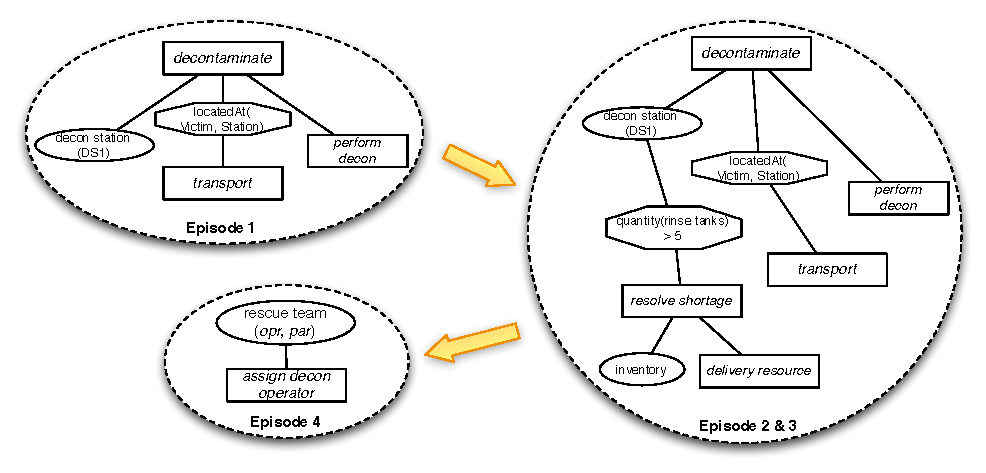
\includegraphics[width=5.8in]{local_scopes_dm.pdf} 
	\caption{The local scopes of $DM$ in four episodes}
	\label{fig:local_scopes_dm}
\end{figure}

Figure \ref{fig:dependencies_ep1} shows the dependency network between actions in the collaborative activity after Episode 1. Similarly, we can construct the dependency networks for all the other three episodes.

\begin{figure}[htbp] %  figure placement: here, top, bottom, or page
	\centering
	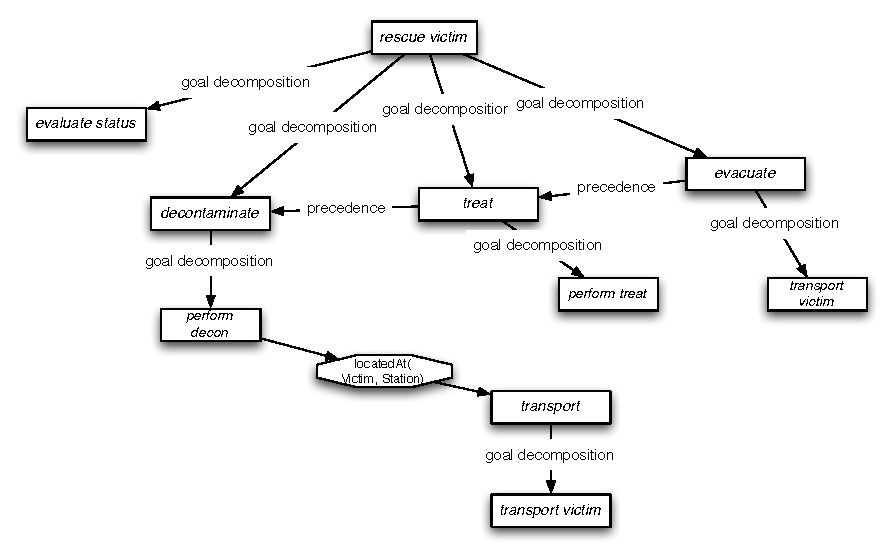
\includegraphics[width=5.8in]{dependencies_ep1.pdf} 
	\caption{The dependency network after Episode 1}
	\label{fig:dependencies_ep1}
\end{figure}
% subsection analyzing_the_characteristics_of_awareness (end)

\subsection{Analyzing the development of awareness} % (fold)
\label{sub:analyzing_the_development_of_awareness_}
In our conceptual model, we argue that the development of awareness at the team level usually entails multiple transactions through which actors' individual awareness processes are connected as developmental trajectories. To understand the development of awareness in the scenario, we perform a detailed interaction analysis in each episode. The interaction analysis focuses on identifying how the awareness information is passed through the actors in each episode. This section reports the results of the interaction analysis.

\subsubsection{Episode 1: Goal activation} % (fold)
\label{ssub:episode_1_goal_activation}
 Episode 1 shows an example of how an initial event can trigger the actor to activate the goal to perform an action, and lead to top-down decomposition of the action. During the development of the action, more awareness information is generated and more actors are participated into the action. Figure \ref{fig:episode_1_interaction} shows the developmental trajectory of awareness in Episode 1.

The trajectory starts with the fireman's report on the discovery of the new victim. This initial event is then received by the victim manager $VM$ in an awareness transaction, which triggers $VM$'s individual awareness process. During the individual awareness process, $VM$ activates the goal that the victim needs to be rescued, which leads to the decision to decomposes the action to rescue the victim into sub-actions, and performance of the action to evaluates the status of the victim, which further leads to $VM$'s adoption of the goals to decontaminate, treat, and evacuate the victim. $VM$ then passes the adoption of the goals to the corresponding actors $DM$, $MM$, and $TM$ respectively through awareness transactions. Upon Upon receiving the event to activate decontamination, $DM$ starts the individual awareness process that leads to her commitment to performing the action, and further elaborates the action. The results of $DM$'s individual awareness processes generate new awareness information about the activation of the goal to transport the victim, which is then passed to $TM$. In a similar way, $TM$ triggers the individual awareness process and passes the activation of the goal to perform transportation task to the driver $DR1$.

\begin{figure}[htbp] %  figure placement: here, top, bottom, or page
   \centering
   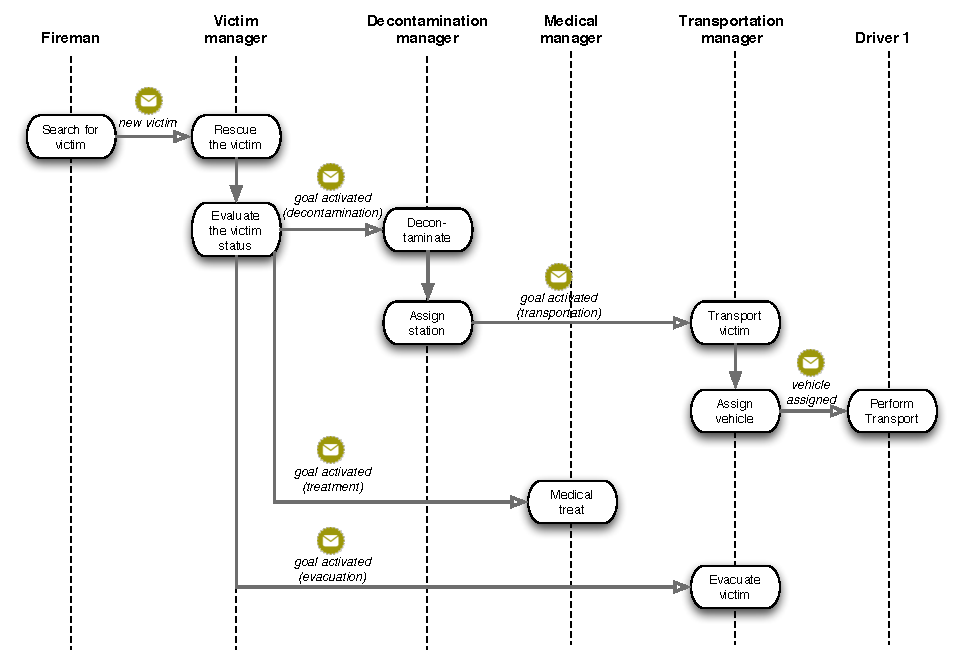
\includegraphics[width=5.8in]{episode_1_interaction.pdf} 
   \caption{Developmental trajectory in Episode 1}
   \label{fig:episode_1_interaction}
\end{figure}
% subsubsection episode_1_goal_activation (end)

\subsubsection{Episode 2: Plan development} % (fold)
\label{ssub:episode_2_plan_development}
Episode 2 shows an example of the opportunistic plan development during the action performance. Although the action to resolve resource shortage is not a required subsidiary component in the initial plan of to rescue the victim, it is later added to the plan because of the problem of a resource is identified during the performance of the action. However, the developmental trajectory in this episode is very similar to Episode 1 as it demonstrates how the awareness information is propagated as the top-level goal is decomposed into subgoals (Figure \ref{fig:episode_2_interaction}).

\begin{figure}[htbp] %  figure placement: here, top, bottom, or page
   \centering
   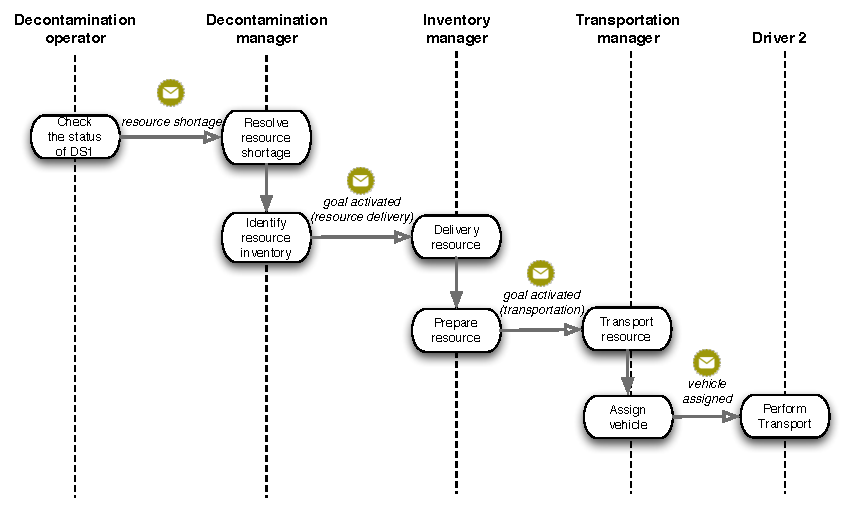
\includegraphics{episode_2_interaction.pdf} 
   \caption{Developmental trajectory in Episode 2}
   \label{fig:episode_2_interaction}
\end{figure}
% subsubsection episode_2_plan_development (end)

\subsubsection{Episode 3: Role transfer} % (fold)
\label{ssub:episode_3_responsibility_transfer}
Unlike the first two episodes, Episode 3 demonstrates the developmental trajectory of the awareness as how the effect of one action can cascade to the other actions because of the dependencies among them (Figure \ref{fig:episode_3_interaction}). 

Episode 3 starts with the event indicating the rescue vehicle with the driver $DR1$ encounters a mechanical breakdown, as the driver is on the way to pick up the victim. The driver reports the problem as the initial event and passes it to $TM$. During the individual awareness process, $TM$ first infers that because of the vehicle breakdown, and the fact that all the drivers are currently in duty, the action to transport the victim has to be delayed. $TM$ expresses this interpretation as a new piece of awareness information. Because the $DM$'s action to decontaminate the victim depends on the transportation action, the awareness information generated by $TM$ is passed to $DM$ through an awareness transaction. In the similar way, $DM$'s interpretation on the delay of decontamination action is passed to $VM$ due to the dependency between the rescue action and the decontamination action. 

\begin{figure}[htbp] %  figure placement: here, top, bottom, or page
   \centering
   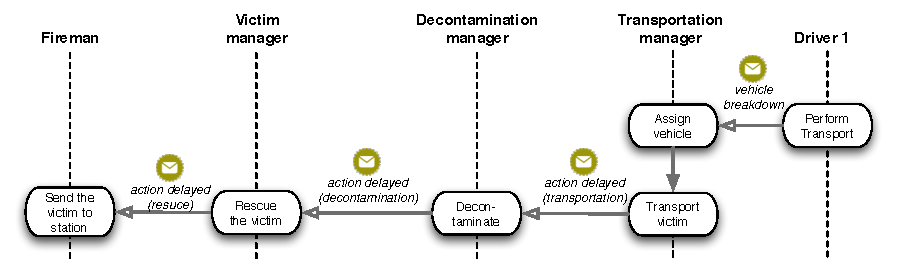
\includegraphics[width=5.8in]{episode_3_interaction.pdf} 
   \caption{Developmental trajectory in Episode 3}
   \label{fig:episode_3_interaction}
\end{figure}
% subsubsection episode_3_responsibility_transfer (end)

\subsubsection{Episode 4: Opportunistic re-planning} % (fold)
\label{ssub:episode_4_opportunistic_re_planning}
Episode 4 shows how one action can be performed using different plans in different situations. Triggered by the initial event, the action has to be opportunistically re-planned to adapt to the changing environment. In the re-planning process, a number of awareness information is derived and distributed around the actors (Figure \ref{fig:episode_4_interaction}).

\begin{figure}[htbp] %  figure placement: here, top, bottom, or page
   \centering
   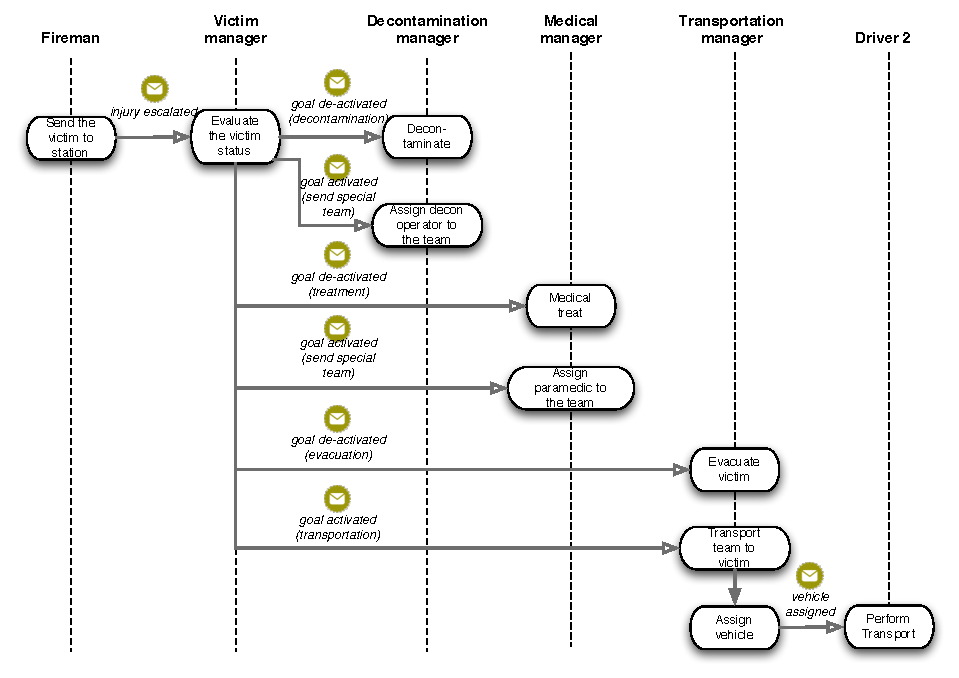
\includegraphics[width=5.8in]{episode_4_interaction.pdf} 
   \caption{Developmental trajectory in Episode 4}
   \label{fig:episode_4_interaction}
\end{figure}
% subsubsection episode_4_opportunistic_re_planning (end)
\subsubsection{Discussion} % (fold)
\label{ssub:discussion}
The interaction analysis of the four episodes demonstrates the characteristics of the development of collaborative awareness in our conceptual model:

\begin{enumerate}
	\item The developmental trajectories of awareness in these episodes clearly show how the awareness knowledge is socially constructed across multiple actors. As the initial event is sent to the team, it is interpreted by an actor who then expresses his/her interpretation of the event as new awareness information and pass it to other actors through awareness transactions. In this way, the awareness knowledge is undergoing continuous construction as the initial awareness information is interpreted and enriched by multiple actors.
	\item These episodes show good examples of how the development of awareness is coupled with the development of the collaborative activity. On one hand are the initial events triggering the development of the collaborative activity, and on the other hand are the changes to the collaborative activity by the actors generate new awareness information. It is within this recursive cycle between the development of awareness and the collaborative activity that the situation is built up.
\end{enumerate}
% subsubsection discussion (end)
% subsection analyzing_the_development_of_awareness_ (end)
% section understanding_the_awareness_phenomena_in_the_scenario (end)

\section{Simulation of the knowledge updating process} % (fold)
\label{sec:simulating_the_knowledge_updating}
The goal of this section is to validate the knowledge updating process within the context of the scenario. To achieve this goal, we simulate the development of the four episodes described in previous section in our prototype system, the EDAP platform, i.e. how the PlanGraph is updated by the \emph{Knowledge Updating Module}, driven by the set of events occur in the episodes. The results of the simulation can then be used to analyze the expressiveness of the PlanGraph model to characterize the awareness phenomena in collaborative activities. 

In general, the simulation is conducted in three steps:

\begin{enumerate}
	\item First, we engineer the knowledge base to model knowledge about all the actions, recipes, and actors that are described in the four episodes. For example, Figure \ref{fig:example_recipes_in_scenario} shows the two recipes associated with the action to rescue the victim.
	\begin{figure}[htbp] %  figure placement: here, top, bottom, or page
   		\centering
   		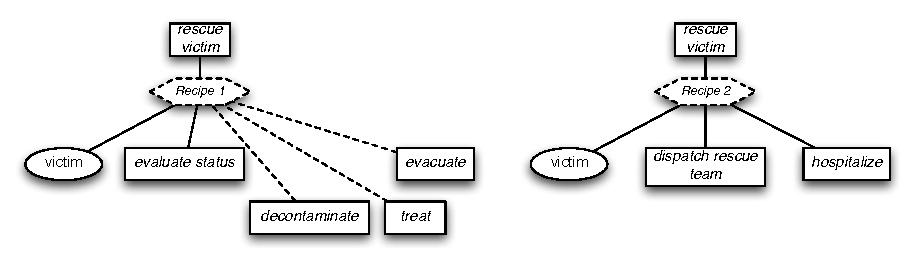
\includegraphics[width=5.8in]{example_recipes_in_scenario.pdf} 
   		\caption{Example recipes in the scenario}
   		\label{fig:example_recipes_in_scenario}
	\end{figure}
	\item Then, we develop an event simulator to input the events that occur in the episodes to the EDAP server. The event simulator is a simple command line tool that reads a pre-defined script recording the sequence of events that are described in the four episodes. At a given time interval, the event simulator emits one event from the sequence and sends it to the \emph{Event Publishing Service} in the EDAP server via HTTP request. The events are generated based on the interaction analysis in previous section, where each piece of awareness information identified in the interaction analysis is represented as an event. Appendix \ref{app:event_description} shows the four sequences of events generated for the simulation.
	\item As we described in Section \ref{sub:service_oriented_modules}, each of the events received by the \emph{Event Publishing Service} is then passed to the \emph{Knowledge Updating Module} to update the PlanGraph model. We persist the PlanGraph during each step in the database for analysis.
\end{enumerate}

\subsection{The simulation process} % (fold)
\label{sub:the_simulation_process}
Here we report the simulation results of the development of the PlanGraph model in the four episodes, which shows the capability of the system to keep track of the event-driven development of the collaborative activity in the scenario.

\subsubsection{Episode 1} % (fold)
\label{ssub:episode_1}
In Episode 1, the first event sent to the system is an event reporting that a new victim has been found by the fireman ($E1$). The event has an event type \emph{`NewVictim'} and has several key attributes (e.g. id, detection time, name, location, radiation level, injury information, etc.). 

In response to this event, the \emph{Knowledge Updating Module} performs the four-step knowledge updating process.

\begin{enumerate}
	\item First, the system attempts to associate with any existing entities in the PlanGraph model. Because this is the start of the activity, the PlanGraph is empty at the moment and no association can be found.
	\item Second, the system checks whether the event can lead to changes towards the action performance or trigger new action in the assessment step. In our knowledge base, we store an association rule that indicates that every \emph{`NewVictim'} will activate the action to rescue it. Following this activation rule, a new action node \emph{`rescue victim'} is added to the PlanGraph as the root node representing this new action to rescue the victim.
	\item After the assessment, the system finds that a new action has been added to the PlanGraph, which triggers the elaboration process. The system searches the knowledge base to find a recipe for the \emph{`rescue victim'} action. In our knowledge base, we have two recipes that are associated with the \emph{`rescue victim'} action and the system chooses the first one that represents the normal workflow to construct the default plan of the action. During the elaboration process, the \emph{`victim'} parameter is assigned with the value stored in the event. The \emph{`evacuate status'} action is added to the plan. Because the rest of the subsidiary actions (\emph{`decontaminate'}, \emph{`treat'}, \emph{`evacuate'}) are optional, i.e. whether they should be added to the plan depends on the result of \emph{`evacuate status'} action, the recipe selection stops. In addition to the recipe selection and parameter binding, the elaboration step also involves searching for the actors who might be potentially intended to or capable of performing the action. By retrieving this knowledge from the knowledge base, the system believes that the victim manager $VM$ is potentially intended to perform the action and have the capability to perform the \emph{`evacuate status'} action. This is used to update the corresponding \emph{`Intentions'} and \emph{`Capabilities'} attributes attached with the PlanGraph nodes.
	\item Because the event does not indicate any state change on current actions, the propagation step is skipped.
\end{enumerate}

Figure \ref{fig:plangraph_ep1_e1} shows the PlanGraph after the knowledge updating process on the first event ($E1$) in Episode 1.

\begin{figure}[htbp] %  figure placement: here, top, bottom, or page
	\centering
	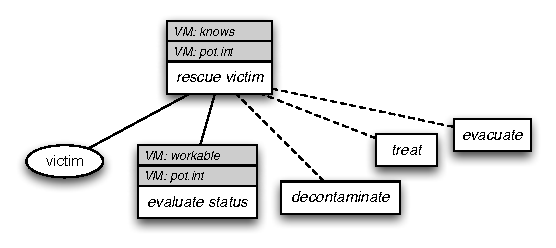
\includegraphics{plangraph_ep1_e1.pdf} 
	\caption{PlanGraph after $E1$ in Episode 1}
	\label{fig:plangraph_ep1_e1}
\end{figure}

The second event ($E2$) in Episode 1 is an internal event generated by the victim manager $VM$ to indicate the intention that ($int.th$) the \emph{`decontaminate'} action is performed, based on the result of the \emph{`evacuate status'} action. This intention event has several key attributes, including the actor's id ($VM$), the action he intends to perform (\emph{`decontaminate'}), and the intention type ($int.th$).

\begin{enumerate}
	\item As the system receives this event $E2$, the system first attempts to associate it with any existing entities in the PlanGraph model. Because this is an intention event, the system traverses through the PlanGraph to search for any match between the \emph{`decontaminate'} action mentioned in the event and the action nodes in the PlanGraph. When the system is able to find such a match, the system uses the information in the event to update $VM$'s intention level on it.
	\item During the assessment step, the system could not find any applicable association rules.
	\item Because the \emph{`decontaminate'} action is now added to the PlanGraph as a new action, the system searches the knowledge base to find a recipe for the \emph{`decontaminate'} action, and use it to elaborate the PlanGraph. Because the system does not have knowledge about how to identify the parameter \emph{`decontamination station'} of the \emph{`decontaminate'} action, the PlanGraph cannot be further elaborated. Besides, the system believes that the decontamination manager $DM$ has potentially intention to perform the \emph{`decontaminate'} action and knows how to perform the action. This is used to update the corresponding \emph{`Inentions'} and \emph{`Capabilities'} attributes attached with the PlanGraph nodes.
	\item Because the event does not indicate any state change on current actions, the propagation step is skipped.
\end{enumerate}

The $E3$ and $E4$ are very similar to $E2$, as they are also internal events generated by the victim manager $VM$ to indicate the intention that ($int.th$) the \emph{`treat'} and the \emph{`evacuate'} action is performed, based on the result of the \emph{`evacuate status'} action. We skip the details here, and Figure \ref{fig:plangraph_ep1_e4} shows the PlanGraph after these events are processed.

\begin{figure}[htbp] %  figure placement: here, top, bottom, or page
	\centering
	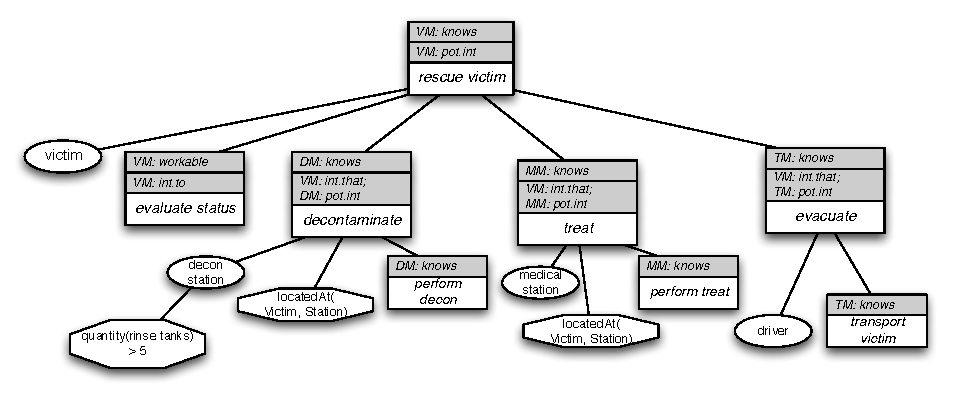
\includegraphics[width=5.8in]{plangraph_ep1_e4.pdf} 
	\caption{PlanGraph after $E4$ in Episode 1}
	\label{fig:plangraph_ep1_e4}
\end{figure}

Events $E5$, $E6$ are generated by the decontamination manager $DM$ in the process of elaborating the action to decontaminate the victim. The system processes these events and elaborate the PlanGraph model in the similar way as the previous events. Finally, the event $E7$ is generated by the transportation manager $TM$ to further elaborate the action to transport the victim to the decontamination station. We skip details about these events as well since the system's reasoning processes on them are very similar to previous ones. Figure \ref{fig:plangraph_ep1_e7} shows the PlanGraph after all the events in Episode 1 are processed.

\begin{figure}[htbp] %  figure placement: here, top, bottom, or page
	\centering
	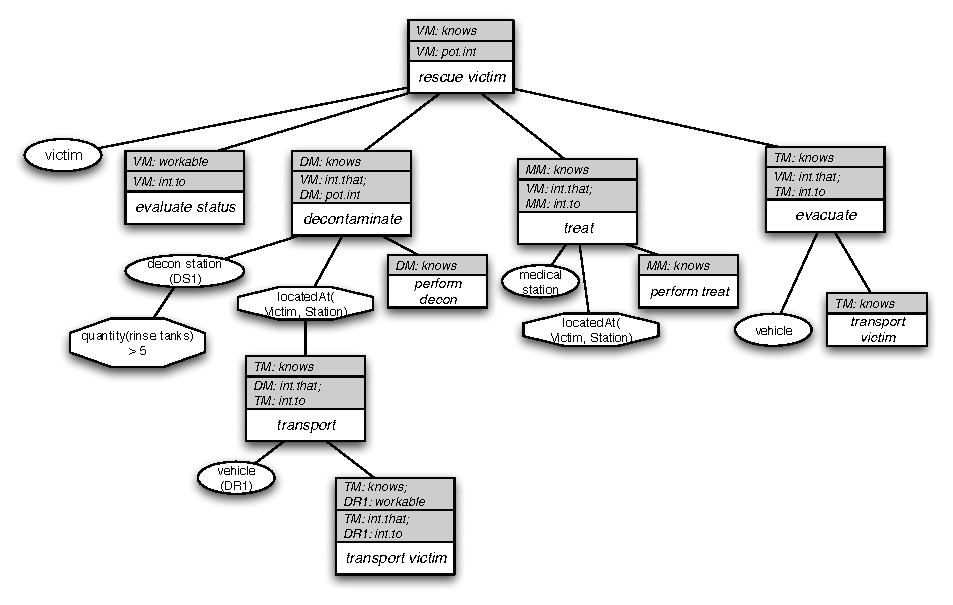
\includegraphics[width=5.8in]{plangraph_ep1_e7.pdf} 
	\caption{PlanGraph after Episode 1}
	\label{fig:plangraph_ep1_e7}
\end{figure}
% subsubsection episode_1 (end)

\subsubsection{Episode 2} % (fold)
\label{ssub:episode_2}
In Episode 2, the first event sent to the system ($E1$) is a resource event reported by an operator at $DS1$, where the decontamination of the victim will be performed. The event shows that the quantity of available rinse tanks in DS1 is running low. The four-step knowledge updating process that is triggered by this event is summarized as follow:

\begin{enumerate}
	\item In the beginning, the system associates the event with the \emph{`decon station'} parameter under the \emph{`decontaminate'} action, as it indicates the value change of an attribute (i.e. quantity of rinse tanks) of the station, and updates the corresponding values of the parameter.
	\item Second, the system checks whether the event can lead to state changes of the entities in the PlanGraph model. By evaluating the conditions associated with the parameter, the system finds that the condition that the quantity of the rinse tanks should be above 5 can no longer be satisfied because of this event. As a result, a new derived event is generated by the system to indicate the state change of this condition (from \emph{`holding'} to \emph{`open'}).
	\item During the elaboration step, since the condition is no longer holding, the system searches the knowledge base to find any action that can be performed to satisfy the condition. In our knowledge base, we have an action \emph{`resolve resource shortage'} that can be used to satisfy the condition, and therefore the system add the action to the PlanGraph and load the recipe to perform the action. The system applies the initial intention $pot.int$ and capability $knows$ of the $DM$ to this new action. Because the system does not have knowledge about how to identify the parameter \emph{`inventory'}, the PlanGraph cannot be further elaborated.
	\item Because a state change event has been derived in the assessment step, the system attempts to predict future state changes in the field of work in the propagation step. A Bayesian network is constructed based on the current PlanGraph model and used to reason how likely the other entities in the PlanGraph will be impacted by the initial state change. After the Bayesian network-based reasoning, the system finds that the state change of this condition (from \emph{`holding'} to \emph{`open'}) will lead to the failing of the \emph{`decon station'} parameter, which may be further propagated to the upper-level \emph{`decontaminate'} and \emph{`rescue'} actions.
\end{enumerate}

Figure \ref{fig:plangraph_ep2_e1} shows the PlanGraph after the knowledge updating process on the first event ($E1$) in Episode 2, and Figure \ref{fig:eventchain_ep2_e1} shows the event chain generated by the system in the process.

\begin{figure}[htbp] %  figure placement: here, top, bottom, or page
	\centering
	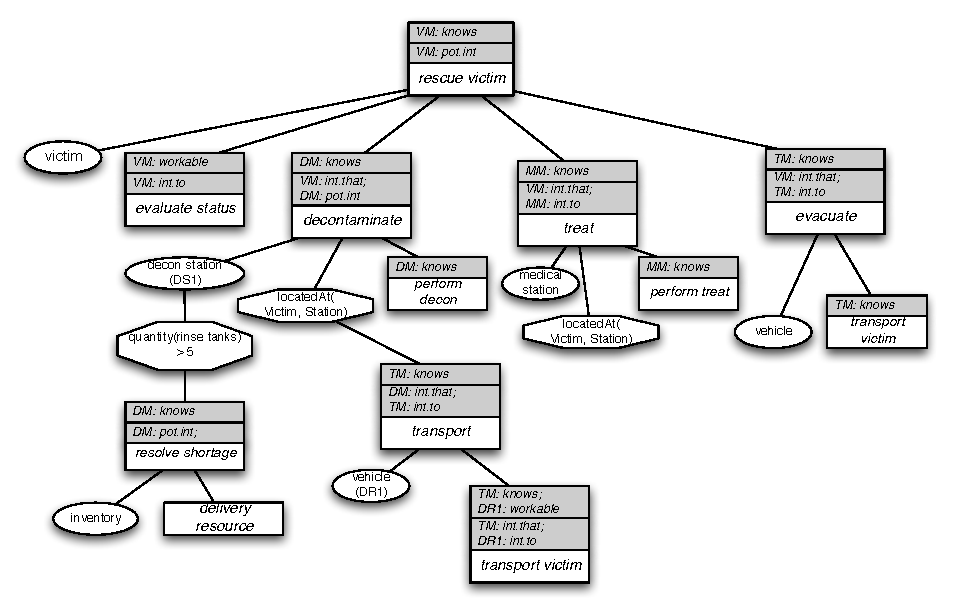
\includegraphics[width=5.8in]{plangraph_ep2_e1.pdf} 
	\caption{PlanGraph after $E1$ in Episode 2}
	\label{fig:plangraph_ep2_e1}
\end{figure}

\begin{figure}[htbp] %  figure placement: here, top, bottom, or page
	\centering
	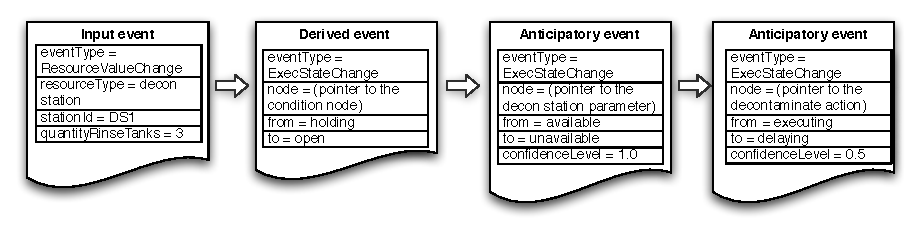
\includegraphics[width=5.8in]{eventchain_ep2_e1.pdf} 
	\caption{Event chain after $E1$ in Episode 2}
	\label{fig:eventchain_ep2_e1}
\end{figure}

The following steps in Episode 2 are developed in the same way as the goal activation process in Episode 1. The decontamination manager $DM$ identifies the \emph{`inventory'} parameter, and then activates the goal to deliver the resource from the inventory to the station $DS1$. The inventory manager then works on the \emph{`deliver resource'} action by preparing the resource and activates the goal to transport the resource to the station. The transportation manager then further elaborates the transportation action. Figure \ref{fig:plangraph_ep2} shows the PlanGraph after all the events in Episode 2 are processed.

\begin{figure}[htbp] %  figure placement: here, top, bottom, or page
	\centering
	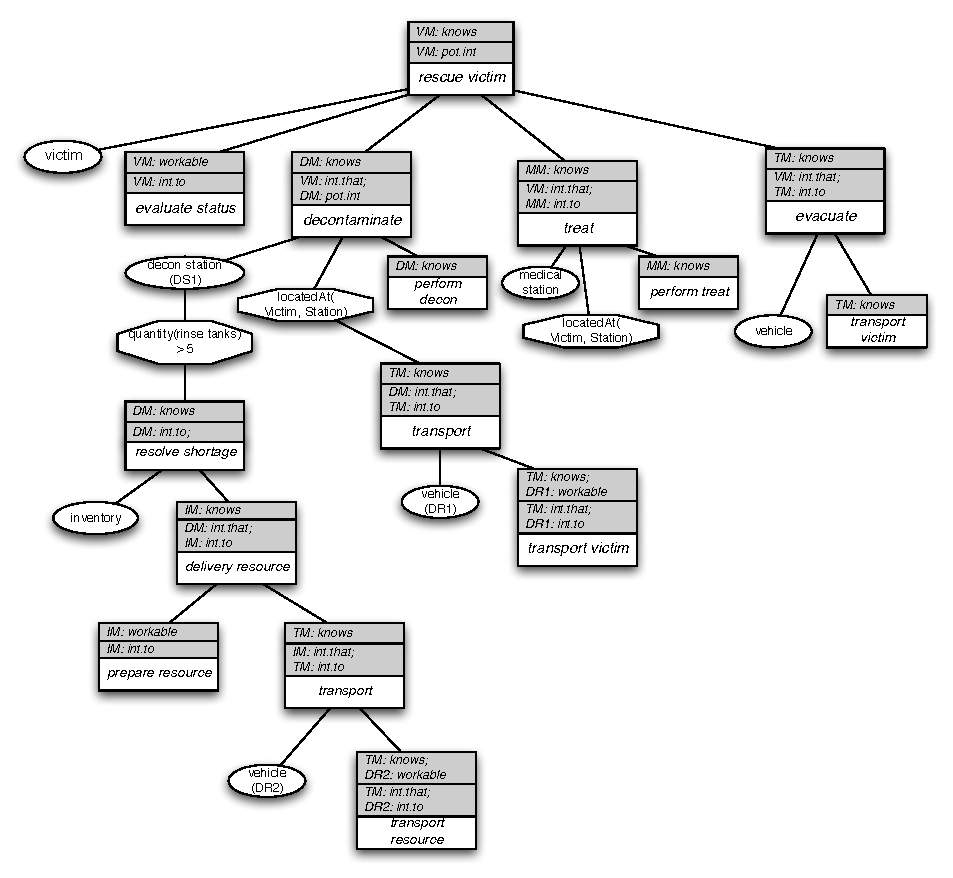
\includegraphics[width=5.8in]{plangraph_ep2.pdf} 
	\caption{PlanGraph after Episode 2}
	\label{fig:plangraph_ep2}
\end{figure}
% subsubsection episode_2 (end)

\subsubsection{Episode 3} % (fold)
\label{ssub:episode_3}
Episode 3 happens after driver $dr_1$ starts the action \emph{`transport victim'} and is on the way to pick up the victim. It is an external event indicating a status change of the rescue vehicle with driver $dr_1$, i.e. it encounters a mechanical breakdown. The event has an event type \emph{`ResourceStatusChange'} and carries information about the driver, the vehicle, and the current status of the vehicle. The knowledge updating process performed on this event by the system is described as follow.

\begin{enumerate}
	\item When the event is sent to the system, the system attempts to associate with any existing entities in the PlanGraph model. Because this is an external event indicating an attribute change on a resource, the system traverses through the PlanGraph to search for any match between the resource (\emph{`vehicle'}) mentioned in the event and the nodes in the PlanGraph. When the system is able to find such a match, the system uses the information in the event to update the value attached to the parameter (\emph{`vehicle'}).
	\item Then the event is further processed in the assessment step. A simple assessment rule is applicable in this case, i.e. if the status of the rescue vehicle is changed to breakdown, the parameter that is assigned with this resource becomes unavailable. As a result, a new state change event \emph{`ExecStatChange'} on the execution state of the parameter is derived.
	\item As nothing can be done by the system to fix this problem by searching the knowledge base, the elaboration is done with nothing added to the PlanGraph.
	\item Because a state change event has been derived in the assessment step, the system attempts to predict future state changes in the field of work in the propagation step. After the Bayesian network-based reasoning, the system finds that the execution state of the $dr_1$'s action to transport the victim (\emph{`transport victim'}) is changed from \emph{executing} to \emph{failing}, and a new anticipatory event describing this state change is generated, and added to the output event chain. Furthermore, the state change is propagated to the higher level \emph{`transport'} action with a confidence level of 0.5, as the system infers that the action is likely to be impacted, meanwhile the problem can be resolved by assigning another vehicle to perform the \emph{`transport victim'} action.
\end{enumerate}

As we can see in the knowledge updating process, the initial event is augmented into an event chain with four events (Figure \ref{fig:eventchain_ep3_e1}): the original external event $E1$, the derived event describing the execution state change of the parameter \emph{`vehicle'}, and the two anticipatory event predicting the execution state change event on the action \emph{`transport victim'} and the \emph{`transport'} action. The processing of $E1$ in Episode 1 shows the capability of the system to enrich the original event by performing reasoning on the PlanGraph.

\begin{figure}[htbp] %  figure placement: here, top, bottom, or page
	\centering
	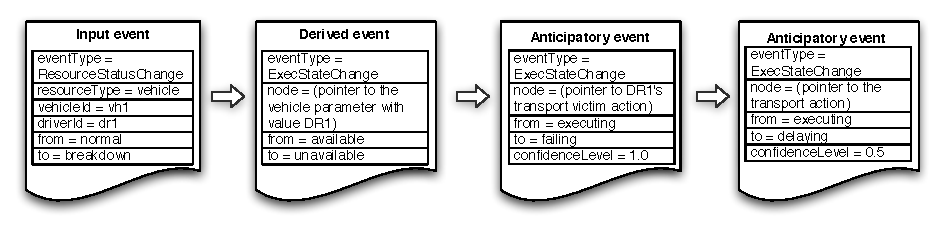
\includegraphics[width=5.8in]{eventchain_ep3_e1.pdf} 
	\caption{Event chain after $E1$ in Episode 3}
	\label{fig:eventchain_ep3_e1}
\end{figure}

The following events $E2$, $E3$, and $E4$ are the internal events that are contributed by the transportation manager ($TM$), decontamination manager ($DM$), and victim manager ($VM$) respectively. These events are used to express the corresponding actors' interpretation on the initial event $E1$. As receiving $E1$, the $TM$ first attempts to fix the problem by assigning another driver to the \emph{`transport victim'} action. However, because all the drivers are currently in duty, the $TM$ cannot find a driver to perform the action until a later time. As a result, the $TM$ generates $E2$ to confirm the state change of the \emph{`transport'} action that was previously inferred by the system. This new event $E2$ is then received by the $DM$, and then $DM$ further derives another event $E3$ to express her belief that the \emph{`decontaminate'} will also be delayed because of $E2$. In the similar way, $VM$ generates the other event $E4$ to propagate the state change. 

The processing of these events allow the system to update the event chain starting with $E1$ using human actors' interpretation, and in this way the event propagation tree can be generated. Figure \ref{fig:eventchain_ep3_e4} shows the active event propagation chain that is derived from the event propagation tree, spanning from $E1$ to $E4$.

\begin{figure}[htbp] %  figure placement: here, top, bottom, or page
	\centering
	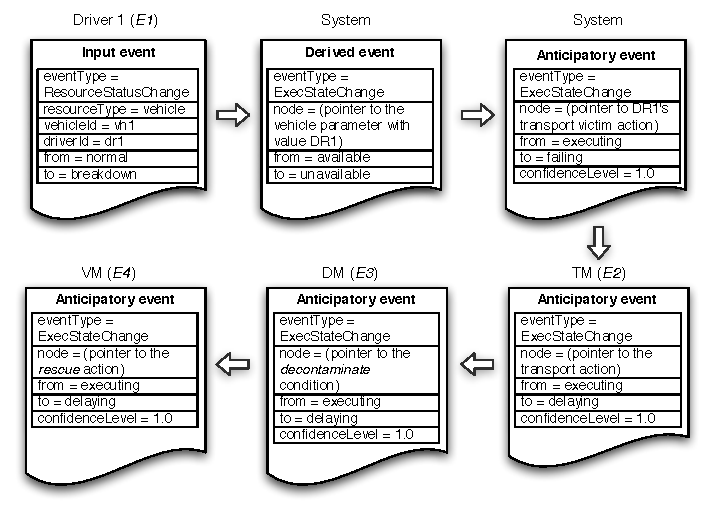
\includegraphics{eventchain_ep3_e4.pdf} 
	\caption{Active event propagation chain after $E4$ in Episode 3}
	\label{fig:eventchain_ep3_e4}
\end{figure}

The last event $E5$ in Episode 3 indicates the fireman's reaction to the situation developed through $E1$ to $E4$. Although delivery of the victim is not in the scope of the fireman's responsibility, she can help fix the problem by directly sending the victim to the decontamination station $DS1$. By receiving $E5$, the system updates the PlanGraph by revising the plan of the \emph{`transport'} action: (1) first the fireman's intention to perform the \emph{`transport'} action is updated in the \emph{Intentions} attribute of the action node during the association step, (2) the value of the \emph{`vehicle'} parameter is now replaced by the vehicle assigned to the fireman, (3) and then the fireman's action to send the victim, i.e. \emph{`send victim'} is added to the \emph{`transport'} action as a sub-action. Figure \ref{fig:plangraph_ep3} shows the PlanGraph after all the events in Episode 3 are processed.

\begin{figure}[htbp] %  figure placement: here, top, bottom, or page
	\centering
	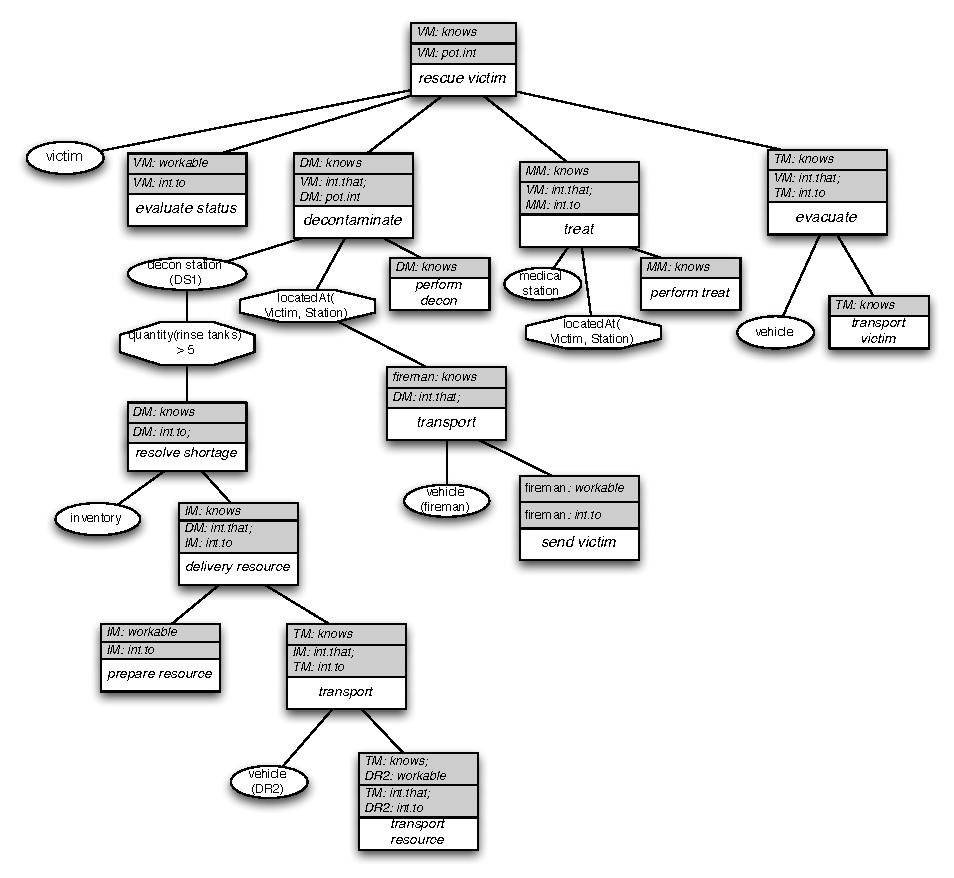
\includegraphics[width=5.8in]{plangraph_ep3.pdf} 
	\caption{PlanGraph after Episode 3}
	\label{fig:plangraph_ep3}
\end{figure}
% subsubsection episode_3 (end)

\subsubsection{Episode 4} % (fold)
\label{ssub:episode_4}
Episode 4 starts with an event $E1$ that indicates the attribute change of a victim, i.e. the injury information is changed. The system associates this event with the \emph{`victim'} parameter under the \emph{`rescue'} action, and updates the attribute storing the injury information. However, such descriptive information cannot be directly interpreted by the system, all the following three steps of the knowledge updating process is skipped. 

The event $E1$ is then interpreted by the victim manager $VM$, who evaluates the changing situation of the victim and decides that because of the serious injury, the original plan to rescue the victim has to be replaced with a new plan. A series of events ($E2$, $E3$, $E4$, $E5$, and $E6$) are then generated by the $VM$ to indicate the change of plan. The system updates the knowledge by removing and adding corresponding actions from the PlanGraph in the association step. During the elaboration step, the system retrieves recipes for the newly added actions and applies default knowledge about intentions and capabilities from the knowledge base. Figure \ref{fig:plangraph_ep4_e6} shows the PlanGraph after the planning events generated by the $VM$ have been processed.

\begin{figure}[htbp] %  figure placement: here, top, bottom, or page
	\centering
	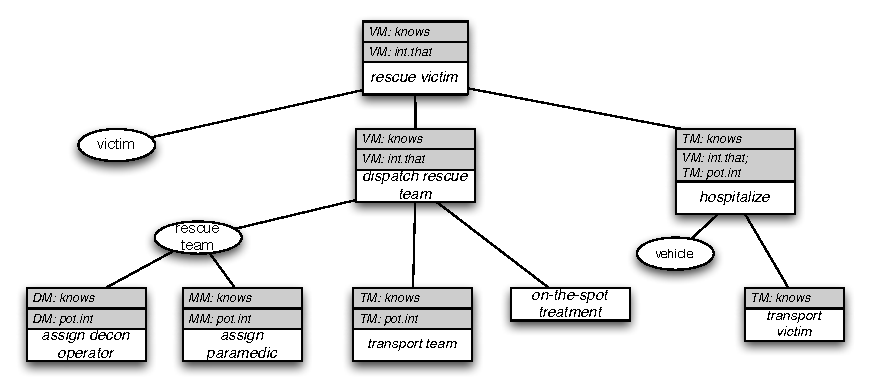
\includegraphics{plangraph_ep4_e6.pdf} 
	\caption{PlanGraph after $E6$ in Episode 4}
	\label{fig:plangraph_ep4_e6}
\end{figure}

After these events are distributed to the corresponding actors ($E2$ and $E5$ for the $DM$, $E3$, $E5$ for the $MM$, and $E4$, $E5$ and $E6$ for the $TM$), these actors interpret them, perform actions in the new plan, and generate new events ($E7$ from the $DM$, $E8$ from the $MM$, and $E9$ from the $TM$) that are then used to update the system's knowledge. The knowledge updating processes triggered by these events are similar to some cases in previous episodes, so we skip the details and shows the final PlanGraph after they are processed in Figure \ref{fig:plangraph_ep4}.

\begin{figure}[htbp] %  figure placement: here, top, bottom, or page
	\centering
	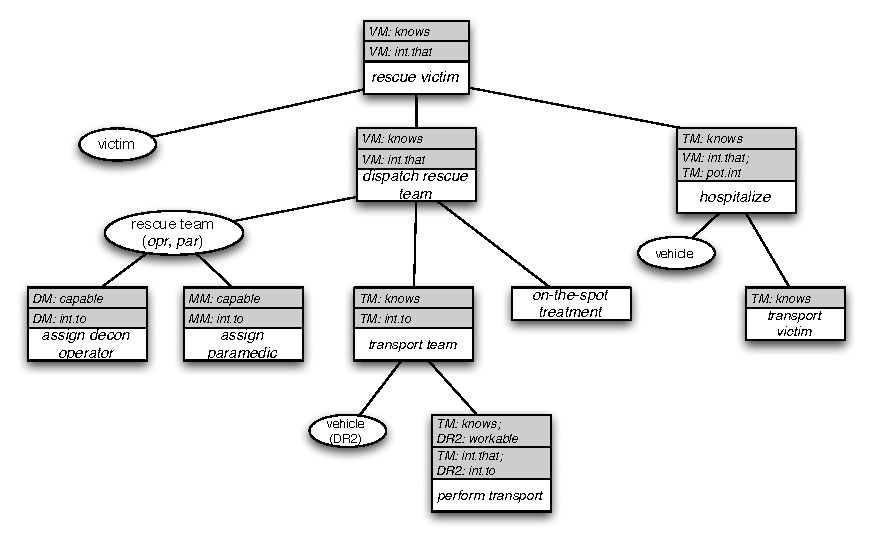
\includegraphics{plangraph_ep4.pdf} 
	\caption{PlanGraph after Episode 4}
	\label{fig:plangraph_ep4}
\end{figure}
% subsection episode_4 (end)
% subsection the_simulation_process (end)

\subsection{Analyzing the awareness phenomena} % (fold)
\label{sub:analyzing_the_awareness_phenomena}
We use the local scopes and dependency networks generated in the simulation process to analyze the three essential characteristics of the awareness as we described in our conceptual framework (Section \ref{sec:awareness_requirements}).  

\subsubsection{Partiality of individual awareness} % (fold)
\label{ssub:partiality_of_awareness}
The first characteristic of awareness in our conceptual model is the \emph{partiality} of individual awareness. The idea is that, since each actor only engages in a small set of actions in a complex, collaborative environment, the actor does not need to fully understand the whole situation. Instead, the information that an actor should be aware of is only partial as it is related to the actions within the actor's local scope of work.

To analyze the partiality of individual awareness in the simulation, we compare the magnitudes of the whole collaborative activity with the local scopes of the victim manager $VM$, the decontamination manager $DM$, the transportation manager $TM$, and the medical manager $MM$. We choose the four actors because they are involved in all the four episodes. The magnitude is defined as the total number of entities (i.e. actions, resource, and actors) in the local scope or the whole collaborative activity. The chart in Figure \ref{fig:partiality_of_awareness_case} shows the counting results. As we can see from the chart, the total number of entities in the collaborative activity (with an average of 20) is much greater than the number of entities in any of the actors' local scopes (the average is 5.5 for $VM$, 6.25 for $DM$, 3.5 for $MM$, and 6.75 for $TM$). From Episode 1 to Episode 2, we can see the whole activity can grow significantly in a collaborative activity, but each actor's local scope is relatively small, and hence much more manageable for the actor.

\begin{figure}[htbp] %  figure placement: here, top, bottom, or page
	\centering
	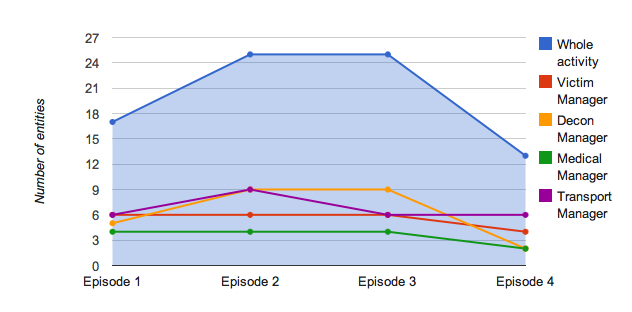
\includegraphics[width=5.8in]{partiality_of_awareness_case.jpg} 
	\caption{Numbers of entities in local scopes}
	\label{fig:partiality_of_awareness_case}
\end{figure}
% subsubsection partiality_of_awareness (end)

\subsubsection{Compatibility of awareness} % (fold)
\label{ssub:compatibility_of_awareness}
The second characteristic of awareness is that the actors' individual awareness needs to be coordinated so as to achieve the compatibility that is collectively needed for the overall team to perform the collaborative task successfully. The requirement for compatible awareness among multiple actors can be accounted for by two characteristics of the collaborative activity: the overlaps between local scopes of work, and the dependencies across local scopes.

To examine the compatibility of awareness, we construct the dependency network from the PlanGraph after Episode 2, and map the different entities in the dependency network into the corresponding actor's local scopes. Figure \ref{fig:dependencies_ep2} shows the visualization of the mapping result. The arrows in the figure indicate the dependency relations between entities, and the shapes in dotted lines with different colors show the local scopes of different actors. The similar mapping results can be generated for the other three episodes, however here we only focus on the Episode 2 as the activity after Episode 2 is the one with the highest level of complexity.

\begin{figure}[htbp] %  figure placement: here, top, bottom, or page
	\centering
	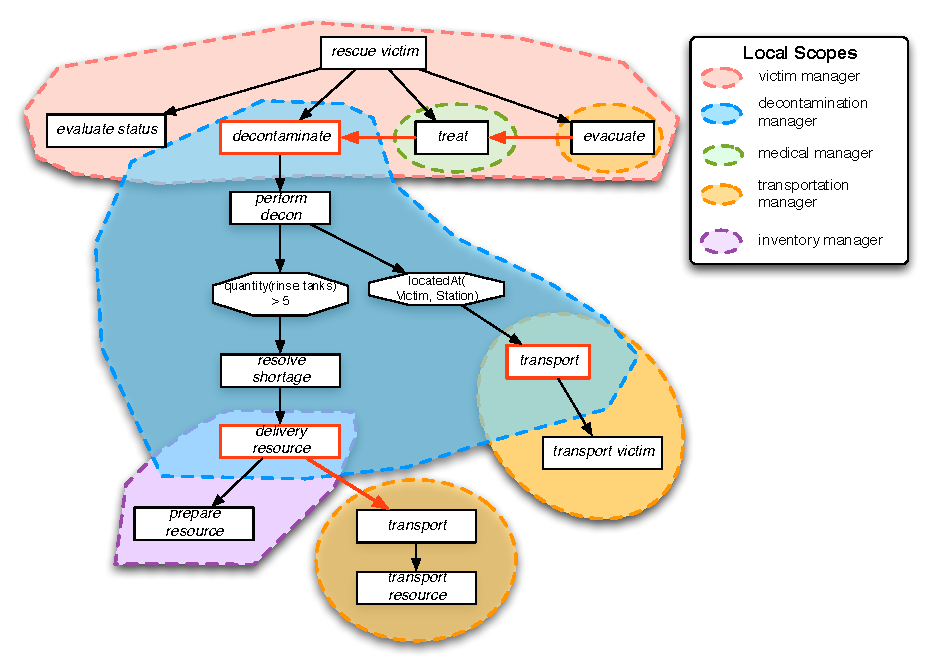
\includegraphics[width=5.8in]{dependencies_ep2.pdf} 
	\caption{Dependency network in Episode 2 with local scopes}
	\label{fig:dependencies_ep2}
\end{figure}

From this figure, we can clearly see both the overlaps between local scopes of work, and the dependencies across local scopes. 

\begin{enumerate}
	\item The entities with the red stroke are the boundary objects that are shared by two overlapping local scopes. For example, the \emph{`delivery resource'} action is a shared object between the decontamination manager $DM$ and the inventory manager $IM$. On one hand, the $DM$ has the intention that the \emph{`delivery resource'} action is performed as it is a subsidiary action for the \emph{`resolve shortage'} action. On the other hand, the $IM$ intends to perform the \emph{`delivery resource'} action because the action is within her responsibility. 
	\item The arrows in red highlight the dependency relations that cross the boundary of two local scopes, i.e. the entity as the depender and the entity as the dependee belong to different actors' local scopes. The temporal dependency relation between the \emph{`decontaminate'} and the \emph{`treat'} action is such an example, as these two actions belong to the decontamination manager and the medical manager respectively. Although the two actors' local scopes do not overlap with each other, the execution state of the \emph{`decontaminate'} action can still have impact on the medical manager, because the \emph{`treat'} action can only be performed after the \emph{`decontaminate'} action is done.
\end{enumerate} 
% subsubsection compatibility_of_awareness (end)

\subsubsection{Dynamics of awareness} % (fold)
\label{ssub:dynamics_of_awareness}
Because the local scopes of work, and dependencies are all under continuous change and development in the complex, distributed collaborative activities, the actors' awareness requirement, i.e. the information an actor is aware of, also entails frequent changes. By comparing the local scopes and dependency networks in each step, we can see that how the local scopes and dependency relations are changing as the collaborative activity is developed.

Figure \ref{fig:partiality_of_awareness_case} shows the changing numbers of entities in the local scope for each actor. From the chart, we can see the different actors' local scopes have quite different growing curves as the collaborative activity is developed. 

Figure \ref{fig:dynamics_of_dependencies} shows the changing size of the dependency networks through the four episodes. For each dependency network, we measure the \emph{size} of the network, i.e. total number of edges in a graph; and the \emph{order} of the network, i.e. total number of vertices in a graph. The chart in the figure shows how the size of the dependency networks is changed from Episode 1 to Episode 4.

\begin{figure}[htbp] %  figure placement: here, top, bottom, or page
	\centering
	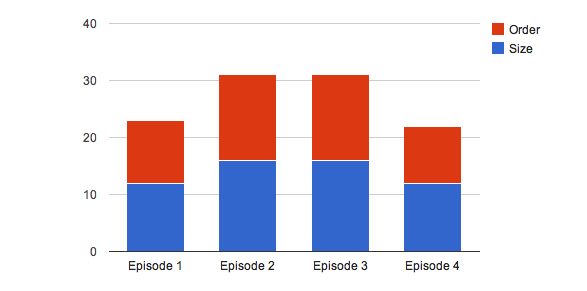
\includegraphics[width=5.8in]{dynamics_of_dependencies.jpg} 
	\caption{Changing dependency networks in the scenario}
	\label{fig:dynamics_of_dependencies}
\end{figure}
% subsubsection dynamics_of_awareness (end)
% subsection analyzing_the_awareness_phenomena (end)
% section simulating_the_knowledge_updating (end)

\section{Promoting awareness in the scenario} % (fold)
\label{sec:promoting_awareness_in_the_scenario}
The four episodes described in Section \ref{sub:event_driven_activity_development} demonstrate the best practices in which the events drive the development of the field of work smoothly in the scenario. However, these best practices are achievable only if the actors in the scenario could successfully develop their awareness in the process. More specifically, these episodes can only happen if the following conditions were satisfied:

\begin{enumerate}
	\item First, the events must be distributed to the right actors at the right time. For example, Episode 1 can only happen if the $VM$ first receives the event $E1$ indicating the discovery of a new victim, and then $E2$, $E3$, and $E4$ are consumed by the $DM$, $MM$, and $TM$ respectively (\emph{Event notification}).
	\item Second, the events must be successfully interpreted by the receivers and hence they are able to make right decisions based on the interpretation (\emph{Event interpretation}). 
	\item Last, the actors must be able to propagate the effect of an event by generating follow-up events that are later consumed by other actors, e.g. Episode 1 works only if $VM$ can propagate the effect of $E1$ by deriving $E2$, $E3$, and $E4$ from it (\emph{Event propagation}).
\end{enumerate}

To satisfy these conditions, awareness support mechanisms become very important. This section analyzes how our awareness promotion approach can be applied in the scenario to enable the satisfaction of these conditions, and compares it with existing awareness support mechanisms.

\subsection{Supporting event notification} % (fold)
\label{sub:supporting_event_notification}
To enable that the events are distributed to the right actors at the right time, event notification mechanisms can be applied. As we described in Section \ref{sec:the_state_of_art}  , existing notification mechanisms rely on event subscriptions that are managed by the human actors. The human actors register the interests in receiving certain kinds of events as subscriptions. The system filters incoming events based on the subscriptions and delivers those matched events to the actors. The event distribution in Episode 1, for example, can be achieved by a set of subscriptions that are managed by different actors. In order to receive $E1$, $VM$ needs to subscribe to all the \emph{`new victim'} events. In order to receive $E2$, $DM$ needs to subscribe to the \emph{`goal activation'} events with the condition that the goal is to decontaminate a victim. Similarly, $MM$ needs to subscribe to the \emph{`goal activation'} events with the condition that the goal is to treat an injured victim to receive $E3$, and $TM$ needs to subscribe to the \emph{`goal activation'} events with the condition that the goal is to evacuate a victim. Table \ref{tab:episode_1_subscriptions} shows the set of subscriptions that need to be managed by the actors to support the event distribution in Episode 1.

\begin{table}[htbp]
\centering
\footnotesize
\begin{tabular}{c>{\raggedright}p{2in}>{\raggedright}p{2.5in}}

\toprule 
\textbf{Event} & \textbf{Receiver} & \textbf{Subscription}\tabularnewline
\midrule 
E1  & Victim manager (VM) & VM needs to subscribe to all the \emph{`new victim'} events\tabularnewline
\midrule 
E2 & Decontamination manager (DM) & DM needs to subscribe to the \emph{`goal activation'} events with
the condition that the goal is to decontaminate a victim\tabularnewline
\midrule 
E3 & Medical manager (MM) & MM needs to subscribe to the \emph{`goal activation'} events with
the condition that the goal is to treat an injured victim\tabularnewline
\midrule 
E4 & Transportation manager (TM) & TM needs to subscribe to the \emph{`goal activation'} events with
the condition that the goal is to evacuate a victim\tabularnewline
\midrule 
E6 & Transportation manager (TM) & TM needs to subscribe to the \emph{`goal activation'} events with
the condition that the goal is to transport a victim to a station\tabularnewline
\midrule 
E7 & Driver (DR1) & DR1 needs to subscribe to the \emph{`resource assignment' }events
with her vehicle as the assigned resource\emph{.}\tabularnewline
\bottomrule

\end{tabular}	
\caption{Subscription-based event distribution in Episode 1}
\label{tab:episode_1_subscriptions}
\end{table}

Alternatively, the local scope-based event notification mechanism as we propose in Section \ref{sec:event_notification_mechanism} provides an approach to distributing the events without explicit event subscriptions by the actors. In our local scope-based approach, the events are distributed to an actor if they are within the actor's local scope. For instance, the event distribution in Episode 1 can be achieved by our approach in the following way:

\begin{enumerate}
	\item Upon receiving $E1$, the system triggers the knowledge updating process in which the system activates the goal to rescue the victim, elaborates the plan to achieve it, associates $E1$ to the \emph{`victim'} parameter, and applies the $VM$'s potential intention to the \emph{`rescue'} action. The detailed explanation of this knowledge updating process can be found at Section \ref{ssub:episode_1}. Then during the notification process, the system finds that $E1$ is associated with the \emph{`victim'} parameter that falls into $VM$'s local scope. As a result, the system believes that $E1$ is relevant and should be notified to the $VM$.
	\item Upon receiving $E2$, the system associates the event with the \emph{`decontaminate'} action, and applies the $DM$'s potential intention to it. During the notification process, the system finds that $E2$ is associated with the \emph{`decontaminate'} action that is within the $DM$'s local scope, and therefore should be distributed to $DM$.
	\item The similar analysis can be performed on the rest of the events in Episode 1, and the system achieves the same effect of distributing these events to the corresponding actors as the subscription-based approach.
\end{enumerate}

Figure \ref{fig:episode_1_ls_distribution} shows how the events in Episode 1 are associated with the entities in the PlanGraph. The different actors' local scopes are also shown in the figure so that we can clearly see how these events fall into the corresponding receivers' local scopes.

\begin{figure}[htbp] %  figure placement: here, top, bottom, or page
	\centering
	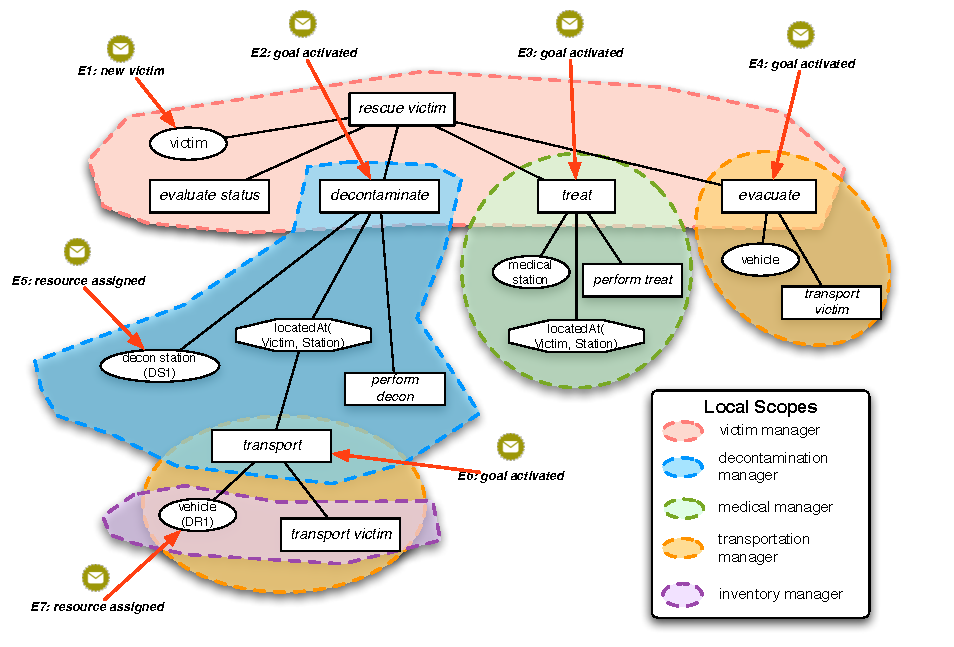
\includegraphics[width=5.8in]{episode_1_ls_distribution.pdf} 
	\caption{Local scope-based event notification in Episode 1}
	\label{fig:episode_1_ls_distribution}
\end{figure}

Comparing with the subscription-based approach, our local scope-based event notification mechanism has two advantages in supporting event distribution: (1) the leverage of system's reasoning to limit the human actor's effort to manage subscriptions within local scopes, and (2) the capability to handle the dynamics of the field of work. We use two concrete cases in the scenario to justify these claims.

\paragraph*{Case 1: Reducing the effort to manage subscriptions} % (fold)
\label{par:case_1_reducing_the_effort_to_manage_subscriptions}
In the first case, we consider the awareness need of the decontamination manager $DM$ in Episode 2. Figure \ref{fig:case_1_dm} shows a portion of the PlanGraph within the $DM$'s local scope and the actions that $DM$'s actions depend on. For example, the \emph{`delivery resource'} action that is within the $DM$'s local scope depends on the inventory manager $IM$'s action to \emph{`prepare the resource'}. The action to transport the victim to the decontamination station depends on the driver $DR1$ to actually perform the transportation operation. 

\begin{figure}[htbp] %  figure placement: here, top, bottom, or page
	\centering
	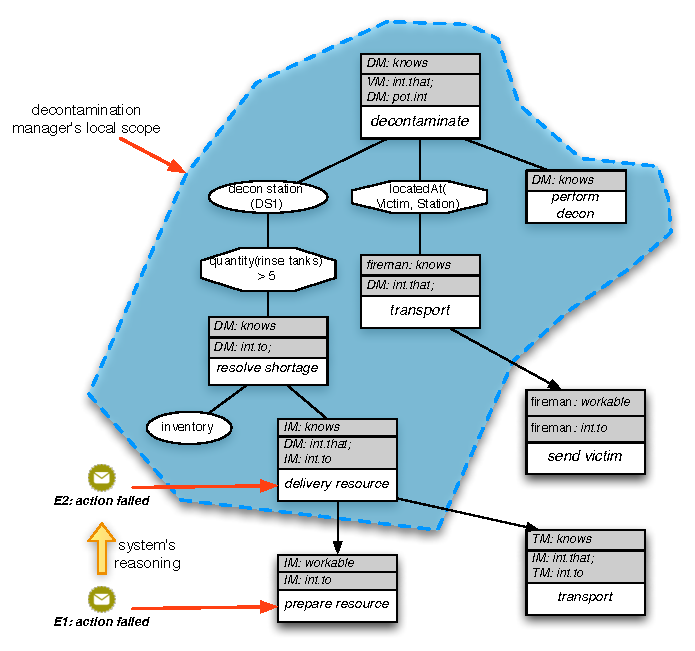
\includegraphics{case_1_dm.pdf} 
	\caption{The $DM$'s local scope in Episode 2}
	\label{fig:case_1_dm}
\end{figure}

Now we consider an event that occurs on an action that is outside the $DM$'s local scope. This event ($E1$) describes that the $IM$'s action to \emph{`prepare the resource'} failed. Although the $IM$'s action to \emph{`prepare the resource'} is outside the $DM$'s local scope, such an event is relevant to the $DM$ because the failing of this action will cause the \emph{`delivery resource'} action that is within the $DM$'s local scope to fail as well. Receiving this event allows the $DM$ to evaluate the impact on her own action, for example, the $DM$ can assign another inventory to supply the resource, or even assign the victim to another decontamination station to avoid the problem. 

In the subscription-based approaches, this means that the $DM$ has to subscribe to the events that may occur on the entities outside her local scope, i.e. the $DM$ needs to manage the subscriptions on the $IM$'s action to \emph{`prepare the resource'}, the $TM$'s action to \emph{`transport'} the resource, and the fireman's action to \emph{`send victim'} to the station.

In our approach, on the other hand, the system performs the reasoning on $E1$ during the knowledge updating process, which allows the system to generate an anticipatory event $E2$ to indicate the potential failing on the \emph{`delivery resource'} action, and attach $E2$ to the event chain along with $E1$. During the local scope-based notification process, because $E2$ falls into $DM$'s local scope, the event chain is then distributed to the $DM$. In this way, the $DM$ only needs to manage the subscriptions within the local scope, e.g. to specify the notification style of the state change on the \emph{`delivery resource'} action, but leaves the task to distribute events outside the local scope to the system.
% paragraph case_1_reducing_the_effort_to_manage_subscriptions (end)

\paragraph*{Case 2: handling the dynamics of awareness need} % (fold)
\label{par:case_2_handling_the_dynamics_of_the_field_of_work}
In the second case, we consider the changing awareness need of the decontamination manager $DM$ in the scenario. As we have shown earlier in Section \ref{ssub:dynamics_of_awareness}, the actors' local scopes change a lot in the development of the collaborative activity. Figure \ref{fig:case_2_dm} shows the changing local scope of $DM$ throughout the four episodes. From Episode 1 to Episode 2, more entities are added to the $DM$'s local scope, and from Episode 3 to Episode 4, the $DM$'s local scope is significantly simplified due to the re-planning on the \emph{`rescue'} action.

\begin{figure}[htbp] %  figure placement: here, top, bottom, or page
	\centering
	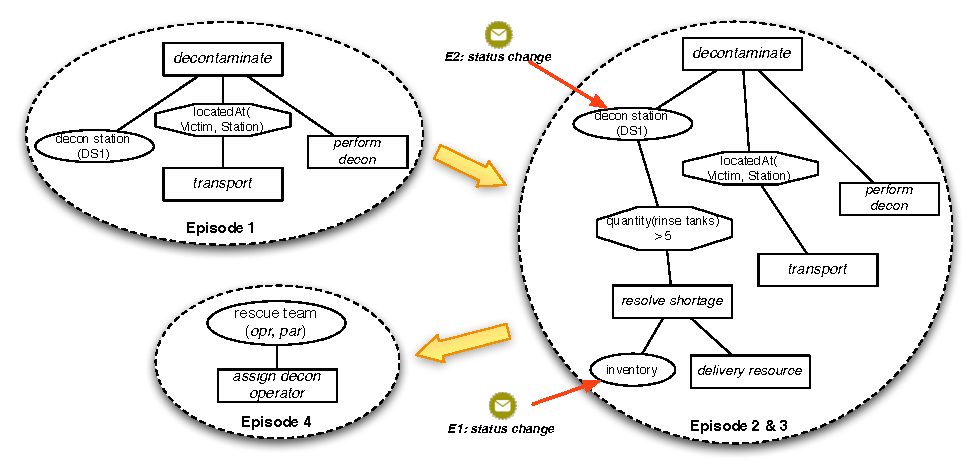
\includegraphics[width=5.8in]{case_2_dm.pdf} 
	\caption{The changing local scope of the $DM$}
	\label{fig:case_2_dm}
\end{figure}

Within the context of the changing local scope, we can easily see how the $DM$'s awareness need is also changed. We consider the event $E1$ that indicates the status change of the inventory that is used to supply the rinse tanks for the station $DS1$. Such an event is only relevant to the $DM$ in the Episode 2 and 3 when it is used to resolve the resource shortage. Similarly, the event $E2$ that indicates the status change of the decontamination station is useful information for the $DM$ in the first three episodes, but it becomes irrelevant in Episode 4 as the $DM$ now only focuses on assigning the operator to the rescue team.

The subscription-based notification mechanisms have difficulties to handle this kind of dynamics. In many existing systems, the subscriptions are pre-defined by the users before the collaborative activity starts. As a result, the subscriptions may be either too narrow to cover all the possible relevant events in the process, or so broad that the system notifies the user the information that has not become relevant yet. To remedy the problem, some systems allow the user to modify the subscriptions on the fly, which provides more flexibility for the users to express their changing needs. However, it requires the users to stop their current work and spend extra effort to explicitly manage the changes in their subscriptions.

Instead, Our local scope-based notification mechanism provides a better solution to handle the dynamics. As the system keeps tracking of the changing field of work, the events are always filtered out based on the current local scopes. For example, if $E1$ is generated during Episode 1, because the system is unable to associate it with any entities in $DM$'s local scope, it is judged as irrelevant to the $DM$. However, if the same event occurs in Episode 2, the system will associate it with the \emph{`inventory'} parameter that is within $DM$'s local scope, and hence it is relevant to $DM$ now.

% paragraph case_2_handling_the_dynamics_of_the_field_of_work (end)
% subsection supporting_event_notification (end)
\subsection{Supporting event interpretation} % (fold)
\label{sub:supporting_event_interpretation}
The event interpretation process plays an important role in the development of collaborative activity throughout the four episodes. On one hand, it allows the actor to consume the perceived events by understanding their meanings within the actor's local scope. Meanwhile, by predicting the future states of entities in the field of work, the actor can generate new events that drive the development of the collaborative activity. 

In the scenario, two types of reasoning tasks can be identified in the event interpretation process:

\begin{enumerate}
	\item \textbf{Backward tracking to understand the origin of an event.} During the event interpretation process, the actors frequently review the historical development of an event to understand where the event comes from. The backward tracking allows the actors to dig into the reasons behind the perceived events to support their decision making. A good example of backward tracking is the fireman's interpretation of $E4$ in Episode 3. In this case, the fireman receives the execution state change event from the victim manager showing that the action to rescue the victim is delayed. Upon receiving this event, the fireman starts the backward tracking to understand that the reason for the occurrence of this event is because the action to decontaminate the victim is delayed, which in turn is because the action to transport the victim to the decontamination station is delayed. By understanding the reason behind the event, the fireman decides to send the victim directly to the decontamination station. Without the backward tracking, it is unlikely that the fireman can change the plan to perform the transportation action that is outside of her responsibility.
	\item \textbf{Forward tracking to evaluate the potential impact of an event.} The forward tracking of an event allows the actors to predict the future states of their actions, which motivates the actors to make changes in the field of work. For instance, the decontamination manager's interpretation of $E1$ in Episode 2 starts with the forward tracking to evaluate the potential impact of the reduced quantity of rinse tanks in the station. During the forward tracking, the decontamination manager infers that the station cannot work properly due to this resource shortage, which in turn will impact the action to decontaminate the victim in the future. The forward tracking of the event motivates the actor to fix the problem caused by the event and activates the new action to resolve the resource shortage.
\end{enumerate}

In our approach, both the backward and forward tracking can be supported through the interlinked event view and activity view as we proposed in Section \ref{sec:supporting_event_interpretation}. 

\paragraph*{Supporting backward tracking} % (fold)
\label{par:supporting_backward_tracking}
The capability of the system to support backward tracking is based on the event propagation tree to keep track of the event development. When an actor generates a new event upon interpreting an existing event, a reference to the current event under interpretation will automatically attached to this new event so that the system can insert it to the event propagation tree. In this way, the system allows the actors to navigate through the event view backward to understand the origin. Figure \ref{fig:backward_chain} shows the sequence of the events that the fireman needs to look into during the interpretation of $E4$ in Episode 3, and how they are linked to the fireman's activity view. 

\begin{figure}[htbp] %  figure placement: here, top, bottom, or page
	\centering
	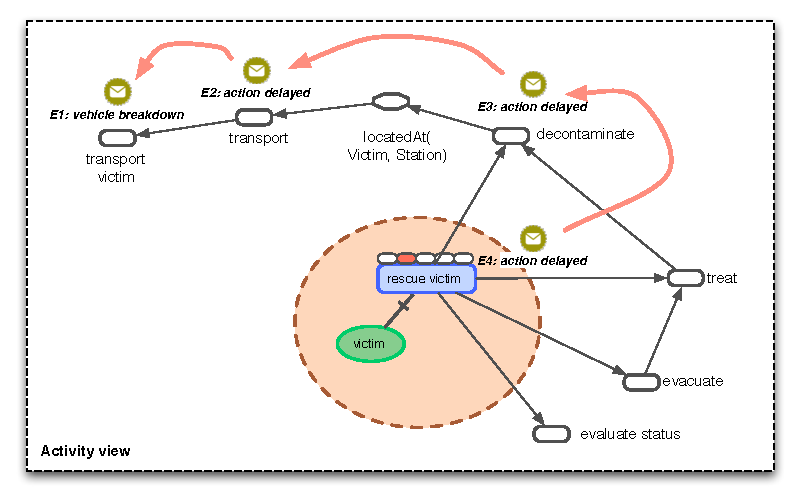
\includegraphics{backward_chain.pdf} 
	\caption{Backward tracking in the interpretation of $E4$ in Episode 3}
	\label{fig:backward_chain}
\end{figure}
% paragraph supporting_backward_tracking (end)

\paragraph*{Supporting forward tracking} % (fold)
\label{par:supporting_forward_tracking}
The forward tracking is supported by the system's capability to perform the reasoning tasks for the human actors. During the knowledge updating process, the system evaluates the consequences of the event and predicts the future states on other activities in the propagation step, and generates the event chain. As we described in Section \ref{ssub:episode_2}, upon receiving $E1$ in Episode 2, the system evaluates the conditions associated with the parameter, and finds that the condition that the quantity of the rinse tanks should be above 5 can no longer be satisfied because of this event. As a result, a new derived event is generated by the system to indicate the state change of this condition (from \emph{`holding'} to \emph{`open'}). Then the system performs the Bayesian network-based reasoning in the propagation step and finds that the state change of this condition (from \emph{`holding'} to \emph{`open'}) will lead to the failing of the \emph{`decon station'} parameter, which may be further propagated to the upper-level \emph{`decontaminate'} action. In this way, the event chain is formed that allows the actors to navigate through the event view forward to predict future states. Figure \ref{fig:forward_chain} shows the sequence of the events that the decontamination manager needs to look into during the interpretation of $E1$ in Episode 2.

\begin{figure}[htbp] %  figure placement: here, top, bottom, or page
	\centering
	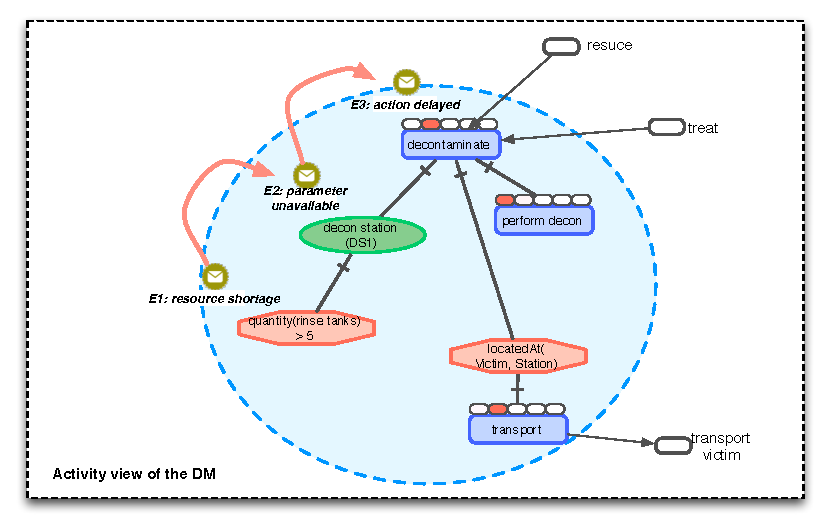
\includegraphics{forward_chain.pdf} 
	\caption{Forward tracking in the interpretation of $E1$ in Episode 2}
	\label{fig:forward_chain}
\end{figure}
% paragraph supporting_forward_tracking (end)
% subsection supporting_event_interpretation (end)

\subsection{Supporting event propagation} % (fold)
\label{sub:supporting_event_propagation}
The social process of event propagation, i.e. the development of awareness involving a series of interactions among multiple actors, can be observed in all the four episodes. The actor who receives the initial event generates his/her own interpretation of the event, which may lead to new goal activated (Episode 1\&2), execution state of existing actions changed (Episode 3), or new plan generated (Episode 4). The actor externalizes the interpretation as new events, which are then received by other actors. These actors build their interpretation on top of the first actor's, and may generate new events that are received by other actors. In this way, as the initial event is propagated to multiple actors, the team awareness is developed.

As we discussed in Section \ref{sec:mediating_event_propagation}, our approach to support event propagation can be analyzed from both the human and the computer's perspectives. From the human perspective, it includes the functionalities to assist human actors to interpret the events built on top of each other's and externalize their own interpretations as new events. From the system's perspective, it focuses on disseminating these events to the actors who are interested in further developing them.

Supporting the human effort in the event propagation process is achieved by the following functionalities provided by our approach:

\begin{enumerate}
	\item First, the system keeps track of the event propagation process and stores the social development history of each event in the corresponding event propagation tree. The visualization of the event propagation tree and active event propagation chain in the event view allows the actors to understand who else have contributed to its development, and whose work can be impacted by the event. Figure \ref{fig:event_chains_in_eps} shows the active event propagation chains that are generated by the system at the end of each episode.
	\item The capability of the human actors to externalize the results of their interpretation as new events is supported by directly manipulating the nodes in the activity view. The EDAP client described in Section \ref{sec:implementation_of_edap_client} demonstrates the functionality to support the externalization. In addition, the interface for the actors to control the visibility of their newly generated events is also supported in the client.
\end{enumerate}

\begin{figure}[htbp] %  figure placement: here, top, bottom, or page
	\centering
	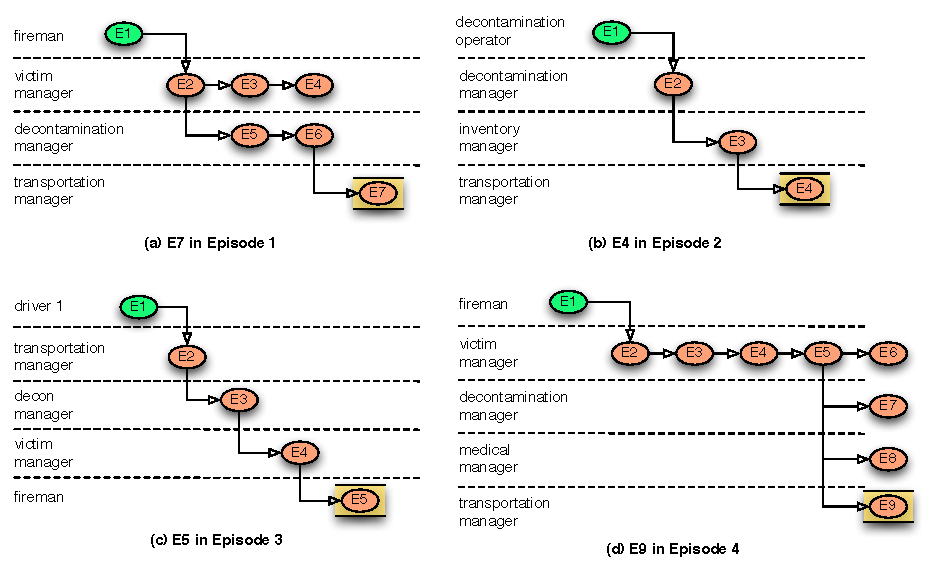
\includegraphics[width=5.8in]{event_chains_in_eps.pdf} 
	\caption{Active event propagation chains in the episodes}
	\label{fig:event_chains_in_eps}
\end{figure}

On the other hand, the capability of system to disseminate these derived events to relevant actors is enabled by the connectivity of local scopes and the local scope-based event notification mechanism. The analysis in Section \ref{sub:compatibility_of_awareness} clearly shows that the entities from different actors' local scopes can be connected with each other, either through the boundary objects in overlapping local scopes or through the dependency relations. The connectivity of local scopes allows the system to propagate the events using the local scope-based event notification mechanism. As long as the new events generated by an actor are associated with the entities that are shared with another actor, or are the dependee of another actor's actions, these events will be propagated to the other actor. 

In the scenario, event propagation through both shard boundary objects and the dependency relations are evident. Figure \ref{fig:two_cases_in_event_proagation} illustrates the two cases of event propagation in the scenario.

\begin{figure}[htbp] %  figure placement: here, top, bottom, or page
	\centering
	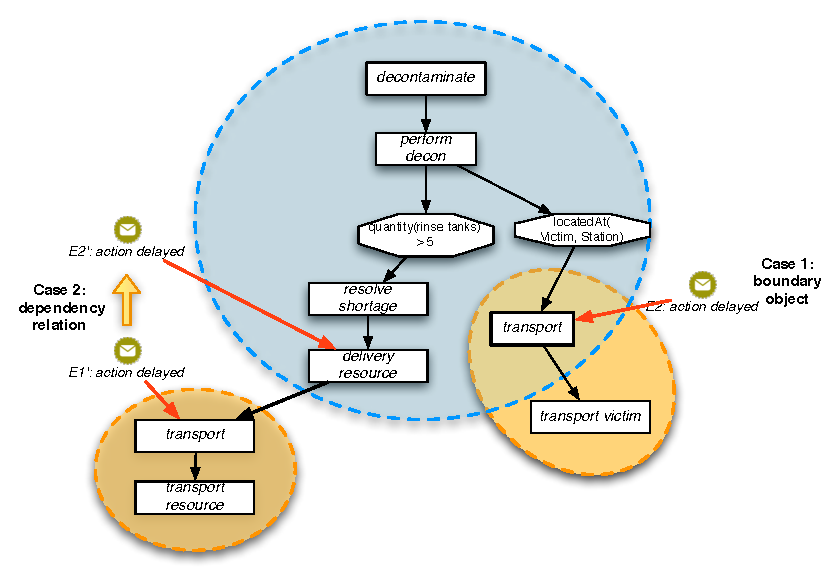
\includegraphics[width=5.8in]{two_cases_in_event_proagation.pdf} 
	\caption{Event propagation through boundary objects and dependency relations}
	\label{fig:two_cases_in_event_proagation}
\end{figure}

The first case happens in Episode 3 when $E2$ is generated by the transportation manager $TM$ to report the delay of the action to \emph{`transport'} the victim. Such an event is the result of the $TM$'s interpretation of the mechanical breakdown of the $DR1$'s vehicle, and is later propagated to the decontamination manager $DM$. In this case, the event propagation happens because the action to \emph{`transport'} the victim is a shared boundary object between both the $DM$ and $TM$'s local scopes. As $E2$ is associated with this boundary object, it falls into the $DM$'s local scope, and as a result, our notification mechanism distributes the event to $DM$.

In the second case, we consider a similar case, but this time the event $E1^\prime$ is generated by the transportation manager $TM$ to report the delay of the action to \emph{`transport'} the resource. In this case, the $TM$'s action to \emph{`transport'} the resource is outside the $DM$'s local scope, however such an event is still relevant to the $DM$ because the dependency relation between the \emph{`transport'} action and the \emph{`prepare the resource'} action. The system performs the reasoning on $E1^\prime$ during the knowledge updating process, which allows the system to generate an anticipatory event $E2^\prime$ to indicate the potential delay on the \emph{`delivery resource'} action, and attach $E2^\prime$ to the event chain along with $E1^\prime$. During the local scope-based notification process, because $E2^\prime$ falls into $DM$'s local scope, it will still be notified to the $DM$. In this case, $E1^\prime$ is propagated to $DM$ because of the dependency relation connecting the two actors' local scopes.
% subsection supporting_event_propagation (end)
% section promoting_awareness_in_the_scenario (end)

\section{Discussion} % (fold)
\label{sec:summary_and_discussion}
This chapter describes a case study in the domain of emergency response to justify our awareness promotion approach. 

In Section \ref{sec:awareness_support_in_emergency_response}, we first describe the characteristics of the emergency response operations and the current status of awareness support in the domain. With the high level complexity and contingency, emergency response fits well into the scope of collaborative activities discussed in this study. The domain of emergency response has foundations in event driven task accomplishment that makes the event-driven awareness support more appropriate. The limitations of existing event-based models as we discussed in previous chapters also exist in the emergency response domain, which motivates our approach.

Section \ref{sec:an_emergency_response_scenario} shows a concrete scenario of the complex, distributed collaborative activity in emergency response. The collaborative activity in this study includes a large number of team workers that engage in a variety of distributed, yet interdependent actions. The four episodes then demonstrate the different types of dynamics that may occur in the scenario, and how the collaborative activity is under continuous development in order to handle the dynamics.

Following the problem scenario, we conduct an analysis of the awareness phenomena in the scenario based on our conceptual model in Chapter \ref{cha:the_conceptual_framework}. The analysis includes a cognitive task analysis and an interaction analysis of the four episodes in the scenario. The former shows the capability of using the conceptual model to understand the major characteristics of collaborative awareness in the scenario, and the latter demonstrates the different developmental trajectories of awareness in the episodes.

To evaluate the expressiveness of the PlanGraph model to represent collaborative activities, and the validity of the knowledge updating processes, we use the EDAP platform to simulate the event-driven development in the four episodes (Section \ref{sec:simulating_the_knowledge_updating}). The development of the PlanGraph model in the four episodes shows the capability of the system to handle the four typical developmental trajectories of collaborative activities as represented by the four episodes respectively. 

In Section \ref{sec:promoting_awareness_in_the_scenario}, we apply the awareness promotion approach in the context of the scenario to analyze the utility of our approach to support the awareness processes in the four episodes. 
\begin{enumerate}
	\item The local scope-based event notification mechanism shows two advantages in supporting event presentation in the scenario: (1) the leverage of system knowledge to limit the human actor's effort to manage subscriptions within local scopes, (2) and the capability to handle dynamics. Because of the partiality of local scopes, our approach reduces the complexity of the event notification problem since the human actors only need to manage subscriptions within their local scopes. On the other hand, the capability of our approach to model dynamics in the field of work provides a more adaptive way to judge the relevance of the events. Instead of relying on pre-defined subscriptions, the relevance of an event is evaluated based on the relation to the up-to-date local scopes in the changing field of work.
	\item Our visualization framework for event interpretation supports two types of reasoning tasks that can be identified in the scenario: (1) backward tracking to understand the origin of an event, and (2) forward tracking to evaluate the potential impact of an event. The former is supported by the capability of the system to keep track of the event development in the knowledge updating process, so that the system can provide the event view to visualize the historical development of an event. The forwarding tracking is supported by the system's capability to perform the reasoning tasks for the human actors. The system's evaluation of an event's consequences and prediction of future states provide suggestions for the human actors to interpret the event. 
	\item Our approach to supporting event propagation includes (1) the functionalities to assist human actors to interpret the events built on top of each others and externalize their own interpretations as new events, and (2) the dissemination of events to relevant actors. The former emphasizes the social aspect of the event propagation process, as how the events are collectively generated and interpreted by multiple actors. The latter is enabled by the connectivity of local scopes in the field of work. The shared boundary objects within the overlapping local scopes and the dependency relations between entities in different actors' local scopes provide the basis for the system to propagate events using the local scope-based event notification mechanism.
\end{enumerate}

% section summary_and_discussion (end)
% chapter case_studies (end)




 

